% vim: set sts=4 et :
\documentclass[prd,preprintnumbers,nofootinbib,twocolumn]{revtex4-1}

\usepackage{amsmath}
\usepackage{amssymb}
\usepackage{booktabs}
\usepackage{graphicx}
\usepackage{multirow}
\usepackage{listings}
\usepackage{xcolor}

\usepackage{textcomp}

\allowdisplaybreaks[1]

%%
%% Setup
%%
% Use the section number in equation tags
\renewcommand{\theequation}{\thesection.\arabic{equation}}
\numberwithin{equation}{section}
\setlength{\parindent}{15pt}

\lstset{
    basicstyle=\ttfamily,
    backgroundcolor=\color{lightgray}
}

%--------+---------+---------+---------+---------+---------+---------+---------+
%
%    Macros
%
%--------+---------+---------+---------+---------+---------+---------+---------+

% references to ...
\def \refeq#1{(\ref{#1})}
\def \refsec#1{sec.~\ref{#1}}
\def \refSec#1{Sec.~\ref{#1}}
\def \refapp#1{app.~\ref{#1}}
\def \reffig#1{fig.~\ref{#1}}
\def \reftab#1{tab.~\ref{#1}}

\def \nn{\nonumber\\}
\def \dis{\displaystyle}

%% tables
\newcommand\tabvsptop{\rule{0pt}{2.6ex}}
\newcommand\tabvspbot{\rule[-1.5ex]{0pt}{0pt}}

%%
%% Comments
%%
\newcommand{\danny}[1]{{\color{purple}{#1}}}
\newcommand{\eos}[1]{{\color{red}{#1}}}   % things to be checked and replaced with EOS results
\newcommand{\fred}[1]{{\color{green}{#1}}}
\newcommand{\todo}[1]{{\color{blue}{ {\bf ToDo: }{#1}}}}
\newcommand{\checked}[1]{{\color{magenta}{ {\bf Checked: }{#1}}}}

%% ----------------------------
%%  Physics, Math, Convenience
%% ----------------------------

% Physics
\newcommand{\wilson}[2][{}]{\mathcal{C}_{#2}^{\mathrm{#1}}}
\newcommand{\op}[1]{\mathcal{O}_{#1}}
\newcommand{\bra}[1]{\big\langle{#1}\big\vert}
\newcommand{\ket}[1]{\big\vert{#1}\big\rangle}
\newcommand{\order}[1]{\mathcal{O}\left({#1}\right)}

% Convenience
\renewcommand{\[}{\big[}
\renewcommand{\]}{\big]}
\renewcommand{\(}{\big(}
\renewcommand{\)}{\big)}
\newcommand{\dd}{{\rm d}}
\newcommand{\para}{\parallel}
\newcommand{\eps}{\varepsilon}
\newcommand{\GeV}{\ensuremath{\mathrm{GeV}}}
%\newcommand{\MeV}{{\si{\MeV}}
\newcommand{\msbar}{\ensuremath{\overline{\rm MS}}}

%% Physics
\newcommand{\alphas}{\alpha_\mathrm{s}}
\newcommand{\alphae}{\alpha_\mathrm{e}}
\newcommand{\gfermi}{G_\mathrm{F}}
\newcommand{\amp}[1]{\mathcal{A}\left({#1}\right)}


%--------------
% math symbols
%--------------

\renewcommand{\Im}[1]{{\rm Im}\left\lbrace{#1}\right\rbrace}
\renewcommand{\Re}[1]{{\rm Re}\left\lbrace{#1}\right\rbrace}

\def \ket#1{ \left| #1 \right\rangle}
\def \brac#1{\left\langle #1 \right|}
\def \averA#1{\left\langle #1 \right\rangle}
\def \aver#1{\langle #1 \rangle}
\def \abs#1{ \left| #1 \right| }
\def \order#1{ {\cal O} \left( #1 \right) }
\def \dslash#1{ #1\!\!\!/}
\def \re{\textrm{Re}}
\def \im{\textrm{Im}}
\def \eps{\varepsilon}
\def \LogGamma{\textrm{LogGamma}}
\def \Amoroso{\textrm{Amoroso}}
\def \vecth{\vec{\theta}}
\def \vecnu{\vec{\nu}}

%-------------
% caligraphic
%-------------

\def \cA{{\cal A}}
\def \cC{{\cal C}}
\def \cF{{\cal F}}
\def \cL{{\cal L}}

%
% effective Lagrangian, operators
%

\def \cLdB1{{{\cal L}_{\Delta B = 1}^{\rm EW}}} % Delta_B = 1 effective Lagrangian
\def \BR{{\cal B}}                               % branching ratio

\def \Op{{\cal O}}
\def \OpQ{{Q}}
\def \OpF{{O}}         % current operator of full theory (Delta_B = 1)
\def \OpE{{\cal O}}    % current operator of effective theory

\def \One{\leavevmode\hbox{\small1\kern-3.6pt\normalsize1}} % unit matrix

%-------------
% differential
%-------------

\newcommand\rmdx[1]{\mbox{d} \, #1 \,}

%--------------------------------
% couplings, scales, observables
%--------------------------------

\def \gS{g_s}              % strong coupling
\def \alS{\alpha_s}        % strong coupling
\def \alE{\alpha_e}        % electro-magnetic coupling
\def \GF{G_F}              % Fermi coupling
\def \LamConf{{\Lambda_{\rm QCD}}}    %  confinement scale
\def \LamConfS{{\Lambda^2_{\rm QCD}}} % (confinement scale)^2

\def \Gaml{{\Gamma_l}}
\def \Game{{\Gamma_e}}
\def \Gammu{{\Gamma_\mu}}

\def \BRl{{{\cal B}_l}}
\def \BRe{{{\cal B}_e}}
\def \BRmu{{{\cal B}_\mu}}

\def \BRll#1#2#3{{\BR(#1) |_{[#2] #3}}}

\def \AFBl{{A_{\rm FB}^l}}
\def \AFBmu{{A_{\rm FB}^\mu}}

\def \FHl{{F_H^l}}
\def \FHe{{F_H^e}}
\def \FHmu{{F_H^\mu}}

%--------
% angles
%--------

\def \thl {{\theta_\ell}}
\def \thK {{\theta_{K}}}
\def \barthl {{\bar{\theta}_l}}
\def \barthK {{\bar{\theta}_{K^*}}}

%--------
% decays
%--------

%
% B -> X + M
%
\def \BtoXM  {\bar{B} \to XM}
%
% b -> scc, B -> J/psi + ...
%
\def \cc{{\bar{c}c}}    % ccbar
\def \bscc   {b \to s + (c\bar{c})}

\def \BJpsiX {\bar{B} \to J/\psi X}
\def \BJpsiXs{\bar{B} \to J/\psi X_s}
\def \BJpsiK {\bar{B} \to J/\psi K}
%
% b -> clv
%
\def \bclv {b\to c l \bar\nu_l}
\def \BXclv  {\bar{B} \to X_c l \bar\nu_l}
%
% b -> s gamma
%
\def \bsgamma {b\to s \gamma}
\def \BXsgamma {\bar{B} \to X_s \gamma}
\def \BtoKastgamma{{ \bar{B} \to K^{\ast} \gamma}}
%
% bs -> ll, B_q -> ll
%
\def \Bstoll{{\bar{B}_s \to \bar{l}l}}
\def \Bstomm{{\bar{B}_s \to \bar{\mu}\mu}}
\def \Bqtomm{{\bar{B}_{d,s} \to \bar{\mu}\mu}}
%
% b -> sll
%
\def \bsll {b\to s \bar{l}l}
\def \BXsll{\bar{B} \to X_s \bar{l}l}

\def \BtoKast{{ \bar{B} \to K^{\ast}}}
\def \B0toK0ast{{ \bar{B}^0 \to K^{\ast 0}}}
%
% excl B->Kll
%
\def \BtoKll{{\bar{B} \to K \bar{l}l}}
\def \BtoKee{{\bar{B} \to K \bar{e}e}}
\def \BtoKmumu{{\bar{B} \to K \bar{\mu}\mu}}
\def \BptoKpll{{B^+ \to K^+ \bar{l}l}}
\def \BmtoKmll{{B^- \to K^- \bar{l}l}}
\def \BneutralKll{{\bar{B}^0 \to K^0 \bar{l}l}}
%%%\def \B0toK0ll{{\bar{B}^0 \to K^0 \bar{l}l}}
\def \BtoKastll{{\bar{B} \to K^\ast \bar{l}l}}
\def \BtoKastmumu{{\bar{B} \to K^\ast \bar{\mu} \mu}}

\def \BmtoKmmumu{{ B^- \to K^- \bar{\mu} \mu}}
\def \B0toK0mumu{{ \bar{B}^0 \to K^0 \bar{\mu} \mu}}
%
% excl B-> K^* (-> K pi) ll
%
\def \BtoKKpill{{ B \to K^\ast (\to K \pi) \bar{l}l}}
\def \BtoKKpimm{{ B \to K^\ast (\to K \pi) \bar{\mu}\mu}}
\def \barB0toKKpill{{ \bar{B}^0 \to \bar{K}^{\ast 0} (\to K^- \pi^+) \bar{l}l}}
\def \B0toKKpill{{ B^0 \to K^{\ast 0} (\to K^+ \pi^-) \bar{l}l}}
\def \BtoKastKpill{{ (\bar{B}^0, B^0)\to (K^{\ast 0},\bar{K}^{\ast 0}) (\to K^\mp \pi^\pm) \bar{l}l}}

%
% Scenario Names
%
\def \SMnu{SM($\nu$-only)}
\def \SM{SM}
\def \SMp{SM+SM$'$}
\def \SMpNine{SM+SM$'$$(9)$}



%--------+---------+---------+---------+---------+---------+---------+---------+
%
%
%
%--------+---------+---------+---------+---------+---------+---------+---------+

\begin{document}

\title{Constraining tensorial and scalar couplings with 
  $B\to K\bar\mu\mu$ and $B_s\to \bar\mu\mu$
}

\author{Frederik Beaujean}
\affiliation{
  C2PAP, Excellence Cluster Universe,\\
  Ludwig-Maximilians-Universit\"at M\"unchen,
  Garching, Germany
}

\author{Christoph Bobeth}
\affiliation{
  Institute for Advanced Study,
  Technische Universit\"at M\"unchen,
  Garching, Germany
}

\author{Stephan Jahn}
\affiliation{
  Excellence Cluster Universe,
  Technische Universit\"at M\"unchen,
  Garching, Germany
}

\date{\today}

\preprint{EOS-2014-??, FLAVOUR(267104)-ERC-??}

\begin{abstract}
  The angular distribution of $B\to K\bar\ell\ell$ ($\ell = e,\,\mu,\,\tau$)
  provides a lepton-forward-backward asymmetry $A_{\rm FB}^\ell$ and a flat
  term $F_H^\ell$ that are both suppressed in the standard model and very
  sensitive to nonstandard tensorial and scalar contributions. We use latest
  experimental results for $\ell = \mu$ in combination with $B_s\to \bar\mu\mu$
  to derive stronger model-independent constraints on tensorial and scalar 
  effective couplings and determine their impact on $B\to K^*\bar\mu\mu$ 
  angular observables. Most notably, the measurement of $F_H^\mu$ provides
  constraints on (pseudo-)scalar couplings and their chirality-flipped 
  counterparts that are complementary to the once from the branching ratio 
  $B_s\to \bar\mu\mu$, which allows to put for the first time upper bounds
  on all four couplings.
\end{abstract}

%
%
%

\maketitle

%
%
%
%--------+---------+---------+---------+---------+---------+---------+---------+
\section{
  Introduction
}

With the first run of data taking by the LHCb Collaboration at the Large Hadron
Collider (LHC), $B$ physics has now also access to rather large samples of
rare $B$-meson decays with branching ratios below the $10^{-5}$. In consequence, 
angular analyses of three- and four-body final states can be used to measure
a larger number of additional observables. Namely rare $B$ decays that are driven
at parton level by flavor-changing neutral current (FCNC) transitions $b\to s
\bar\ell\ell$ constitute valuable probes of the standard model (SM) and provide
constraints on its extensions, especially $B\to K^*(\to K\pi) \bar\ell\ell$, but
also $B\to K \bar\ell\ell$. 

The angular distribution of $B\to K \bar\ell\ell$ in the angle $\theta_\ell$
between the $B$ and $\ell^-$ as measured in the dilepton rest frame
\begin{align}
  \label{eq:ang-distr}
  \frac{1}{\Gamma_\ell} \frac{\mbox{d}\Gamma_{\ell}}{\mbox{d}\!\cos\theta_\ell} & 
  = \frac{3}{4} (1 - F_H^\ell) \sin^2\!\theta_\ell 
  + \frac{1}{2} F_H^\ell
  + A_{\rm FB}^\ell \cos\theta_\ell \,,
\end{align}
normalised to the width $\Gamma_\ell$, has been recently updated with 3 fb$^{-1}$
by LHCb \cite{Aaij:2014tfa} for the mode $B^+\to K^+ \bar\mu\mu$, i.e. $\ell = \mu$,
with unprecedented precision, and the first analysis of $B^0\to K_{S} \bar\mu\mu$
has been reported as well. It provides the lepton-forward-backward asymmetry 
$A_{\rm FB}^\mu$ and the flat term $F_H^\mu$ in CP-averaged form and integrated
over several bins in the dilepton invariant mass $q^2$. Similarly, the CP-averaged
branching ratios, ${\cal B}_\mu = \tau_{B} \Gamma_\mu$,~\cite{Aaij:2014pli}
and the rate CP asymmetry $A_{\rm CP}^\mu$ \cite{Aaij:2014bsa} are also
available from 3 fb$^{-1}$.

Both observables exihibit strong suppression factors for vectorial and dipole
couplings present in the SM, thereby enhancing their sensitivity to tensorial and
scalar couplings \cite{Bobeth:2007dw, Bobeth:2012vn}. A similar enhancement of
scalar couplings compared to helicity-suppressed vectorial couplings of the SM 
is well-known from $B_s\to \bar\mu\mu$. Unfortunately the limited data set of
$B\to K^*(\to K\pi) \bar\ell\ell$ from LHCb \cite{Aaij:2013qta} still does not
allow to perform current angular analysis without the assumption of vanishing
scalar and tensorial couplings in this decay mode. In the future also certain
angular observables in $B\to K^* \bar\ell\ell$ will provide additional constraints
on such couplings, as for example $J_{6c}$ \cite{Altmannshofer:2008dz}
and the linear combinations $(J_{1s} - 3 J_{2s})$ and $(J_{1c} + J_{2c})$ 
\cite{Matias:2012xw, Bobeth:2012vn} as well as at low recoil the experimental
test of the relations $H_T^{(2)} = H_T^{(3)}$ and $J_7 = 0$~\cite{Bobeth:2012vn}. 

Here we exploit current data from $B^+\to K^+ \bar\mu\mu$ and $B_s\to \bar\mu\mu$
to derive stronger constraints then before on tensorial and scalar couplings in
various model-independent scenarios and study their impact on the yet not
measured analogous observables in $B\to K^* \bar\ell\ell$. In \refsec{sec:EFT},
we specify the effective theory of $|\Delta B| = 1$ decays, on which our
model-independent fits are based on. We discuss the dependence of observables
in $B\to K \bar\ell\ell$ and $B\to K^* \bar\ell\ell$ on the tensorial and scalar
couplings in \refsec{sec:observables} and specify also the experimental input
used in the fits. The constraints on tensorial and scalar couplings from the data
are presented for several model-independent scenarios in \refsec{sec:results}.
Technical details on the treatment of theory uncertainties are relegated to
appendices.

%
%
%
%--------+---------+---------+---------+---------+---------+---------+---------+
\section{
  Effective Theory 
  \label{sec:EFT}
}

In the framework of the $|\Delta B| = |\Delta S| = 1$ effective theory 
\begin{align}
  \label{eq:Heff}
  {\cal L}_{\rm eff} & =
   \frac{4 G_F}{\sqrt{2}} \,\frac{\alE}{4 \pi}\, V_{tb}^{} V_{ts}^\ast
       \sum_{\ell = e, \mu,\tau} \sum_i  \wilson[\ell]{i}(\mu_b)  \Op_i + \text{h.c.}
\end{align}
the most general dimension-six flavor-changing operators $\Op_i$ mediating
$b\to s \bar\ell\ell$ are classified according to their chiral structure. 
There are dipole ($i = 7,7')$ and vectorial ($i = 9,9',10,10'$) operators 
\begin{equation}
  \label{eq:SM:ops}
\begin{aligned}
  \Op_{7(7')} & 
  = \frac{m_b}{e}\!\[\bar{s} \sigma^{\mu\nu} P_{R(L)} b\] F_{\mu\nu}\,,
\\
  \Op_{9(9')} & 
  = \[\bar{s} \gamma_\mu P_{L(R)} b\]\!\[\bar{\ell} \gamma^\mu \ell\]\,,
\\[0.1cm]
  \Op_{10(10')} & 
  = \[\bar{s} \gamma_\mu P_{L(R)} b\]\!\[\bar{\ell} \gamma^\mu \gamma_5 \ell\]\,,
\end{aligned}
\end{equation}
further scalar ($i = S,S',P,P'$) operators
\begin{equation}
  \label{eq:scalar:ops}
\begin{aligned}
  \Op_{S(S')} & 
  = \[\bar{s} P_{R(L)} b\]\!\[\bar{\ell} \ell\]\,,
\\[0.1cm]
  \Op_{P(P')} & 
  = \[\bar{s} P_{R(L)} b\]\!\[\bar{\ell} \gamma_5 \ell\]\,,
\end{aligned}
\end{equation}
and tensor ($i = T,T5$) operators
\begin{equation}
  \label{eq:tensor:ops}
\begin{aligned}
  \Op_{T} & 
  = \[\bar{s} \sigma_{\mu\nu} b\]\!\[\bar{\ell} \sigma^{\mu\nu} \ell\]\,,
\\[0.1cm]
  \Op_{T5} & 
  = \[\bar{s} \sigma_{\mu\nu} b\]\!\[\bar{\ell} \sigma^{\mu\nu} \gamma_5 \ell\]\,,
\end{aligned}
\end{equation}
where the notation $\Op_{T5} = i/2\, \varepsilon^{\mu\nu\alpha\beta}
\[\bar{s} \sigma_{\mu\nu} b\]\!\[\bar{\ell} \sigma_{\alpha\beta} \ell\]$ is
also used frequently in the literature. Their respective short-distance couplings,
the Wilson coefficients $\wilson[\ell]{i}(\mu_b)$ are evaluated at the typical
scale of the $b$-quark mass $\mu_b \sim m_b$ and can be modified from SM predictions
in the presence of new physics.

The SM values $\wilson[\ell]{7,9,10}$ are obtained at NNLO \cite{Bobeth:2003at, 
Huber:2005ig} and depend on the fundamental parameters of the top-quark and
$W$-boson masses, as well as on the sine of the weak mixing angle. Moreover,
they are universal for the three lepton flavors $\ell = e,\, \mu,\, \tau$.
All other Wilson coefficients are numerically suppressed or zero: 
$\wilson[SM]{7'} = m_s/m_b\, \wilson[SM]{7}$, $\wilson[SM]{S,S',P,P'} \sim 
{\cal O}(m_b^2/m_W^2)$, and $\wilson[SM]{9',10',T,T5} = 0$. Beyond the SM,
lepton-flavor non-universal effects are possible in principle and have been 
discussed for example recently \cite{Alonso:2014csa, Hiller:2014yaa, Ghosh:2014awa, 
Biswas:2014gga, Hurth:2014vma, Glashow:2014iga, Altmannshofer:2014rta, Hiller:2014abc} in
connection with the measurement of $R_K = {\cal B}_\mu/{\cal B}_e$ in
$q^2 \in [1, 6]$ GeV$^2$ \cite{Aaij:2014ora}, which deviates by $2.6\sigma$
from the SM prediction $R_K^{\rm SM} = 1.00$ \cite{Bobeth:2007dw, Bouchard:2013mia}.

The Wilson coefficients of the four-quark current-current and QCD-penguin
operators as well as of the chromomagnetic dipole operators are set to their
NNLO SM values at $\mu_b = 4.2 \, \mbox{GeV}$ \cite{Bobeth:2003at, Huber:2005ig}.

%
%
%
%--------+---------+---------+---------+---------+---------+---------+---------+
\section{
  Observables and experimental input
  \label{sec:observables}
}

The full dependence of $F_H^\ell$ and $A_{\rm FB}^\ell$ on tensorial and scalar
couplings has been presented in \cite{Bobeth:2007dw, Bobeth:2012vn}, adopting
the effective theory \refeq{eq:Heff}, i.e. neglecting higher dimensional operators
with $\mbox{dim} > 6$. These results imply that for SM values of the effective 
couplings
\begin{align}
  F_H^\ell(q^2)|_{\rm SM} & \propto \frac{m_\ell^2}{q^2}\,, &
  A_{\rm FB}^\ell|_{\rm SM} & = 0 \,.
\end{align}
Hence, for $\ell = e,\, \mu$ both observables are quasi-null tests. 
The $F_H^\ell(q^2)|_{\rm SM}$
is strongly suppressed away from both kinematical endpoints in $q^2$,
except for $\ell = \tau$, \cite{Bobeth:2007dw, Bobeth:2011nj, Bouchard:2013eph}.
Non-zero values
of $A_{\rm FB}^\ell|_{\rm SM}$ can be induced by higher order QED corrections,
which in principle could also give additional $\cos\theta_\ell$ dependence
to the angular distribution~\refeq{eq:ang-distr}, however, currently there is
no solid estimate available for this source of SM background. 

This picture does not change in the presence of new physics contributions to
vectorial and dipole operators $i = 7,7',9,9',10,10'$. On the other hand,
non-vanishing tensorial or scalar contributions are enhanced unless the 
dynamics of NP implies similar suppression factors, i.e., lepton-Yukawa couplings
for $F_H^\ell$ or $\alpha_e$ in the case of $A_{\rm FB}^\ell$. In particular,
$F_H^\ell$ is very sensitive to tensorial couplings whereas $A_{\rm FB}^\ell$ to
the interference of tensorial and scalar couplings.

\begin{figure*}
  \includegraphics[width=.24\textwidth]{plots/pdf/FH-1-6_vs_CT.pdf}
  \includegraphics[width=.24\textwidth]{plots/pdf/FH-15-22_vs_CT.pdf}
  \includegraphics[width=.24\textwidth]{plots/pdf/Br-K-1-6_vs_CT.pdf}
  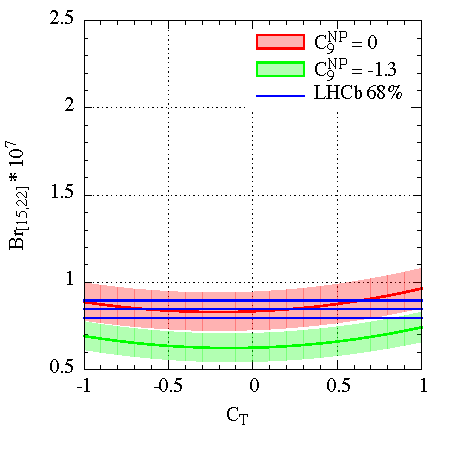
\includegraphics[width=.24\textwidth]{plots/pdf/Br-K-15-22_vs_cT.pdf}
\\
  \includegraphics[width=.24\textwidth]{plots/pdf/Br-Kstar-1-6_vs_CT.pdf}
  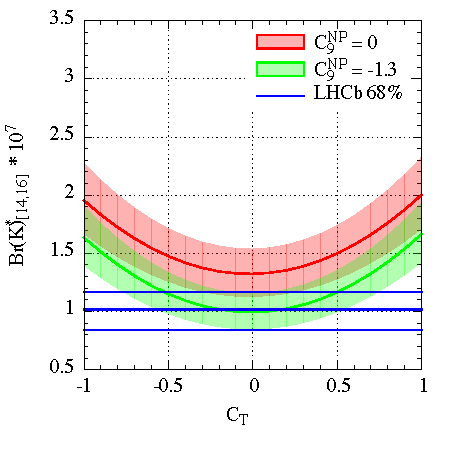
\includegraphics[width=.24\textwidth]{plots/pdf/Br-Kstar-14-16_vs_cT.pdf}
  \includegraphics[width=.24\textwidth]{plots/pdf/Br-Kstar-16-19_vs_CT.pdf}
  \caption{
    \eos{The sensitivity of $F_H^\mu$ [upper row: 1, 2], ${\cal B}(B^+ \to K^+ 
    \bar\mu\mu)$ [upper row: 3, 4] and ${\cal B}(B^0 \to K^{*0} \bar\mu\mu)$
    [lower row] integrated over $q^2$ at low and high $q^2$ to the tensorial
    coupling $\wilson{T}$. The bands represent the theory uncertainties at
    68\% probability. 
    For comparison two values of $\wilson[NP]{9} = 0$ (red) and $\wilson[NP]{9} 
    = -1.3$ (green) are shown together with the 68\% measurements of LHCb (blue).}
  }
  \label{fig:FHvsCT}
\end{figure*}

There are also angular observables $J_i$ in $B\to K^*(\to K\pi)\,
\bar\ell\ell$ with the same properties, i.e. tensorial and scalar contributions
are kinematically enhanced by a factor $\sqrt{q^2}/m_\ell$ over vectorial once 
present in the SM or their respective interference terms. These are $J_{6c}$ 
and the two linear combinations $(J_{1s} - 3 J_{2s})$ and $(J_{1c} + J_{2c})$ 
with explicit formulas given in \refapp{app:BKstarellell}. 
In the limit of vanishing lepton mass one obtains that
\begin{align}
  J_{6c} & \propto 
    \mbox{Re}\big[(\wilson[]{P} - \wilson[]{P'})\, \wilson[\ast]{T} 
                - (\wilson[]{S} - \wilson[]{S'})\, \wilson[\ast]{T5}\big]
\intertext{is sensitive to the interference of tensorial and scalar operators,
  complementary to lepton forward-backward asymmetry of $B\to K \bar\ell\ell$} 
  \label{eq:AFB-dependence}
  A_{\rm FB}^\ell & \propto 
    \mbox{Re}\big[(\wilson[]{P} + \wilson[]{P'})\, \wilson[\ast]{T5} 
                + (\wilson[]{S} + \wilson[]{S'})\, \wilson[\ast]{T}\big]
                \Big/ \Gamma_\ell \,,
\end{align}
i.e., with an interchange of tensorial contributions $T \leftrightarrow T5$.
We note also that $J_{6c}$ contributes to lepton forward-backward asymmetry
of $B\to K^* \bar\ell\ell$ being $\propto (J_{6s} + J_{6c}/2)$. Since
it has to compete with $J_{6s}$ in this observable, a separate measurement of
$J_{6s}$ and $J_{6c}$ is necessary. Further, only tensorial contributions enter
\begin{align}
  (J_{1s} - 3\, J_{2s}) & \propto 
  \left(\ldots |\wilson{T}|^2 + \ldots |\wilson{T5}|^2 \right) \,,
\end{align} 
where the dots indicate different kinematical and form factor dependences.
On the other hand, tensorial and scalar contributions enter
\begin{equation}
\begin{aligned}
  (J_{1c} + J_{2c}) & \propto 
      \ldots \left(|\wilson{T}|^2 + |\wilson{T5}|^2 \right)
\\
  & + \ldots \left(|\wilson{S} - \wilson{S'}|^2 + |\wilson{P} - \wilson{P'}|^2 \right) \,,
\end{aligned}
\end{equation}
which is similar to the dependence of $F_H^\ell$ in $B\to K 
\bar\ell\ell$
\begin{equation}
  \label{eq:FH-dependence}
\begin{aligned}
  F_H^\ell  \propto & \Big[
      \ldots \left(|\wilson{T}|^2 + |\wilson{T5}|^2\right)
\\
  & + \ldots \left(|\wilson{S} + \wilson{S'}|^2 + |\wilson{P} + \wilson{P'}|^2 \right)
  \Big]
  \Big/ \Gamma_\ell \,.
\end{aligned}
\end{equation}
Concerning $F_H^\ell$, the involved kinematical factors --- see \cite{Bobeth:2007dw, 
Bobeth:2012vn} --- are such that tensorial and scalar couplings contribute only 
constructively, apart of cancellations among $\wilson{S(P)}$ and $\wilson{S'(P')}$.
Further, interference terms (in the numerator of $F_H^\ell$) of $(\wilson{T} \times 
\wilson{7,7',9,9'})$ and $(\wilson{P,P'} \times \wilson{10,10'})$ are suppressed
by $m_\ell/\sqrt{q^2}$, but can become relevant in case $\wilson{T} \ll \wilson{7,7',9,9'}$
and $\wilson{P,P'} \ll\wilson{10,10'}$ can overcome this suppression factor,
respectively.

The observables $F_H^\ell$ \refeq{eq:FH-dependence} and $A_{\rm FB}^\ell$
\refeq{eq:AFB-dependence} are measured in the angular
distribution \refeq{eq:ang-distr} of $B\to K \bar\ell\ell$ being normalised to the
decay width $\Gamma_\ell$, whereas $J_{6c}$,  $(J_{1s} - 3\, J_{2s})$ and $(J_{1c} + J_{2c})$
appear in the unnormalised angular distribution of $B\to K^* \bar\ell\ell$.
Hence in the former, uncertainties due to form factors can cancel in part
\cite{Bobeth:2007dw, Bobeth:2012vn}. So-called ``optimised'' versions $S_1$, $M_1$ and
$M_2$ for the low-$q^2$ region have been identified in~\cite{Matias:2012xw} 
for $J_{6c}$,  $(J_{1s} - 3\, J_{2s})$ and $(J_{1c} + J_{2c})$, respectively.
In \refapp{app:BKstarellell} potential normalisations are discussed that
could serve to form optimised observables at high $q^2$ for special cases of
either vanishing chirality-flipped vectorial or tensorial or scalar couplings.
In the most general case, however, there are no optimised observables.
Although form factors do not cancel in this case, it might be
still advantageous to use normalisations, for example when the overall
normalisation of $B\to K^*$ form factors constitutes a major theoretical
uncertainty.

\begin{table*}
\begin{center}
\renewcommand{\arraystretch}{1.4}
\begin{tabular}{lccc}
\hline
Channel & Constraints & Kinematics & Source
\\
\hline \hline
$B_s\to \bar\mu\mu$
& $\int\dd\tau \BR(\tau)$ &  --  & \cite{Aaij:2013aka,Chatrchyan:2013bka,CMS:2014xfa}
\\
\hline
\multirow{2}{*}{${B^+\to K^+ \bar\mu\mu}$}
    & \multirow{2}{*}{$\BR_\mu$}
    & $q^2\in [1,\, 6],\, [14.18,\, 16],\, [> 16]$ GeV$^2$  & \cite{CDF:2012:BKstarll} \\
    &
    &  $\,\,\,\,\, q^2 \in [1.1,\, 6.0],\, [15.0,\, 22.0]$ GeV$^2$  & \cite{Aaij:2014pli} \\
    & $A_{\rm FB}^\mu$
    &  $\,\,\,\,\, q^2 \in [1.1,\, 6.0],\, [15.0,\, 22.0]$ GeV$^2$  & \cite{Aaij:2014tfa} \\
    & $F_{H}^\mu$
    &  $\,\,\,\,\, q^2 \in [1.1,\, 6.0],\, [15.0,\, 22.0]$ GeV$^2$  & \cite{Aaij:2014tfa} \\
    & $A_{\rm CP}^\mu$
    &  $\,\,\,\,\, q^2 \in [1.1,\, 6.0],\, [15.0,\, 22.0]$ GeV$^2$  & \cite{Aaij:2014bsa}    
\\   
\hline
    ${B^0\to K^{\ast 0} \bar\mu\mu}$
    & $\BR_\mu$
    & $q^2\in [1,\, 6],\, [14.18,\, 16],\, [> 16]$ GeV$^2$  & \cite{CDF:2012:BKstarll, Aaij:2013iag,Chatrchyan:2013cda} \\
    & $A_{\rm CP}^\mu$
    &  $\,\,\,\,\, q^2 \in [1.1,\, 6.0],\, [15.0,\, 22.0]$ GeV$^2$  & \cite{Aaij:2014bsa}
\\    
\hline \hline
${B\to K}$ form factors
    & $f_{0,+,T}$   &  $q^2 = 17,\, 20,\, 23$ GeV$^2$  & \cite{Bouchard:2013eph} \\
\hline
\multirow{3}{*}{${B\to K^*}$ {form factors}}
    & $V/A_1$ &  $q^2 = 0$ GeV$^2$  & \cite{Hambrock:2013zya} \\
    & $A_0$   &  $q^2 = 0$ GeV$^2$  & \cite{Khodjamirian:2010vf} \\
    & $V$, $A_1$, $A_{12}$
              &  $q^2 = 15,\, 19.21$ GeV$^2$     & \cite{Horgan:2013hoa}  \\
\hline
\end{tabular}
\renewcommand{\arraystretch}{1.0}
\caption{\label{tab:observables} List of all observables in the various
  exclusive $b\to s \bar\mu\mu$ decays that enter the fits with their
  respective kinematics and experiments that provide the measurements. 
  Lattice results of $B\to K$ form factors are used to constrain their parameters,
  and theoretical constraints on $B\to K^*$ form factors are included. For
  more details see the text and \refapp{app:theory:inputs}.  
}
\end{center}
\end{table*}

To illustrate the sensitivity of $F_H^\ell$ to tensorial couplings, we compare
it in \reffig{fig:FHvsCT} to the one of the branching ratios of $B\to K^{(*)}
\bar\ell\ell$, integrated over low and high $q^2$. The details of the numerical
input and the treatment of uncertainty propagation can be found in \refapp{app:theory:inputs}.
In view of the hint of new physics in $\wilson[NP]{9} < 0$ from recent global analysis of 
$b\to s (\gamma,\, \bar\ell\ell)$ data \cite{Descotes-Genon:2013wba, Altmannshofer:2013foa, 
Beaujean:2013soa, Hurth:2014vma, Altmannshofer:2014rta} we show besides 
$\wilson[NP]{9} = 0$ also predictions for $\wilson[NP]{9} = -1.3$. As can be seen, 
the sensitivity to tensorial couplings is highest for $F_H^\ell$ at high $q^2$, 
also due to a partial cancellation of form factors \cite{Bobeth:2012vn}, 
whereas the one on $\wilson[NP]{9} < 0$ is rather mild, in contrast to that of
the branching ratios. For the latter, ${\cal B}(B\to K^* \bar\ell\ell)$ shows
stronger dependence on $\wilson{T}$ compared to ${\cal B}(B\to K \bar\ell\ell)$
and has some impact on the constraints on tensorial couplings as will be
discussed in \refsec{sec:results}. In consequence, the data on $F_H^\ell$ at
high $q^2$ provides currently the most stringent constraints on the size of 
tensorial couplings. Moreover, the dependence on vectorial couplings is such that 
$\wilson[NP]{9} < 0$ leads to stronger constraints on $\wilson{T}$ than
$\wilson[NP]{9} \approx 0$.

Important additional constraints on scalar couplings come from the branching
ratio of $B_s \to \bar\mu\mu$ as given in \refeq{eq:Br-Bsmumu}. It provides
the most stringent constraints on the moduli $|\wilson{S} - \wilson{S'}|$
and $|\wilson{P} - \wilson{P'}|$ that are complementary to \refeq{eq:FH-dependence}
in $B\to K \bar\ell\ell$ and depends only on the further combination 
$(\wilson{10} - \wilson{10'})$. 

Eventually we also explore the behaviour of derived constraints with respect
to destructive interference with vectorial couplings $\wilson{9,\,10}$. For
this purpose we include also the branching ratio and the rate CP asymmetry
of $B\to K^* \bar\mu\mu$ as it provides additional constraints on the moduli
of vectorial couplings.

In our fit of the effective couplings $\wilson{i}(\mu_b)$, we do not neglect
kinematically suppressed terms in predictions of measured observables as well
as when predicting not yet measured observables. The experimental input of these
observables is listed in \reftab{tab:observables} together with input for the 
$B\to K^{(*)}$ form factors. More details on the latter can be found in 
\refapp{app:theory:inputs}.

%
%
%
%--------+---------+---------+---------+---------+---------+---------+---------+
\section{
  Fits and constraints
  \label{sec:results}
}

As a matter of the fact there are no discrepancies between the latest measurements
for $\ell = \mu$ (throughout this section)
of $F_H^\mu$ and $A_{\rm FB}^\mu$ and their tiny SM predictions. Thus our main objective
is the derivation of stronger constraints on tensorial and scalar couplings, which
are enhanced in both observables compared to vectorial ones. For this purpose,
we will consider several model-independent scenarios, starting from rather
restricted to more general ones, in order to asses the effect of cancellations
among different contributions.

We will start with only tensorial couplings and see that they are well constrained
by $F_H^\mu$ alone. In a second step we consider only scalar couplings in order
to investigate the complementarity of $F_H^\mu$ and $B_s \to \bar\mu\mu$.
Eventually we will consider as a special scenario the SM augmented by dimension
six operators as an effective theory of new physics below some high scale
$\Lambda_{\rm NP}$, much larger than the typical scale of electroweak 
symmetry breaking $v$ in the presence of one scalar doublet under $SU(2)_L$,
as in the SM, i.e. $v \ll \Lambda_{\rm NP}$.

%
%
%--------+---------+---------+---------+---------+---------+---------+---------+
\subsection{Tensorial couplings \label{sec:tensor}}

\begin{table*}
  \renewcommand{\arraystretch}{1.3}
  %\resizebox{\textwidth}{!}{
  \begin{tabular}{c|ccc}
  \hline
  data set
  & only $F_H^\mu$
  & $F_H^\mu$ + other
  & $F_H^\mu$ + other
  \\ 
  set of couplings
  & $\wilson{T,\,T5}$
  & $\wilson{T,\,T5}$
  & $\wilson{T,\,T5,\, 9,\,10}$
  \\
  \hline \hline
  $\mbox{Re}\,\wilson{T}$
  & \eos{$\quad$ $[-0.35,\, 0.20]$ ($[-0.55,\, 0.40]$) $\quad$}
  & \eos{$\quad$ $[-0.20,\, 0.15]$ ($[-0.35,\, 0.30]$) $\quad$}
  & \eos{$\quad$ $[-0.20,\, 0.20]$ ($[-0.40,\, 0.35]$) $\quad$}
  \\
  $\mbox{Im}\,\wilson{T}$
  & \eos{$[-0.25,\, 0.25]$ ($[-0.45,\, 0.45]$)}
  & \eos{$[-0.15,\, 0.15]$ ($[-0.30,\, 0.30]$)}
  & \eos{$[-0.20,\, 0.20]$ ($[-0.35,\, 0.35]$)}
  \\[0.1cm]
  $\mbox{Re}\,\wilson{T5}$
  & \eos{$[-0.25,\, 0.25]$ ($[-0.45,\, 0.45]$)}
  & \eos{$[-0.10,\, 0.20]$ ($[-0.25,\, 0.35]$)}
  & \eos{$[-0.20,\, 0.15]$ ($[-0.35,\, 0.35]$)}
  \\
  $\mbox{Im}\,\wilson{T5}$
  & \eos{$[-0.25,\, 0.25]$ ($[-0.45,\, 0.45]$)}
  & \eos{$[-0.15,\, 0.15]$ ($[-0.30,\, 0.30]$)}
  & \eos{$[-0.20,\, 0.20]$ ($[-0.35,\, 0.35]$)}
  \\
  \hline 
  $|\wilson{T}|$, $|\wilson{T5}|$
  & \eos{$< 0.35$ ($< 0.55$)}
  & \eos{$< 0.25$ ($< 0.35$)}
  & \eos{$< 0.30$ ($< 0.45$)}
  \\
  \hline 
  \end{tabular}
%}
  \renewcommand{\arraystretch}{1.0}
  \caption{
     \label{tab:cTT5:1-dimCLs}
     The constraints on complex-valued $\wilson{T,\,T5}$ --- [upper] 1D-marginalized 
     at 68\% (95\%) probability and [lower] 2D-marginalized --- when using
     measurements of $i)$ only $F_H^\mu$, $ii)$ $F_H^\mu$ and other data in
     \reftab{tab:observables} (except $B_s \to \bar\mu\mu$), and $iii)$ allowing
     also new physics contributions to $\wilson{9,\,10}$ with uniform prior
     \eos{$\mbox{Re},\mbox{Im}(\wilson[NP]{i}) \in [-3,\, 3]$}.
  }
\end{table*}

In a scenario with only tensorial complex-valued couplings $\wilson{T,\, T5}$,
the experimental measurement of $F_H^\mu$ constrains the combination
$|\wilson{T}|^2 + |\wilson{T5}|^2$, up to some small interference of
$\wilson{T}$ with vectorial couplings $\wilson{7,\,7',\,9,\,9'}$. 
The according 68\% (95\%) 1D-marginalized probability intervals are listed in
\reftab{tab:cTT5:1-dimCLs}. As can be seen further in \reftab{tab:cTT5:1-dimCLs},
the constraints become tighter when utilising all observables in
\reftab{tab:observables}, mainly due to the branching ratio of $B\to K^{*} 
\bar\mu\mu$. The latter stronger bounds are driven by the new lattice
results of $B\to K^*$ form factors that yield too high predictions compared
to the measurements~\cite{Horgan:2013pva}. Since tensorial couplings contribute
constructively to ${\cal B}(B\to K^{*}\bar\mu\mu)$ large values are stronger
constrained. In this scenario, the measurements of $A_{\rm FB}^\mu$ does not pose
constraints due to vanishing scalar couplings and we find that the rate 
CP-asymmetries $A_{\rm CP}$ of $B\to K^{(*)} \bar\mu\mu$ do not provide 
constraints, therefore omitting them.

Eventually, we perform a fit with non-zero complex-valued $\wilson{9,\,10}$
by allowing uniform priors for \eos{$\mbox{Re, Im}(\wilson[NP]{i}) \in[-3,\, 3]$},
($i = 9,10$) in order to access the stability of the bounds derived from $F_H^\mu$
against destructive interference. In this case, $F_H^\mu$ by itself still provides 
bounds \eos{$|\wilson{T,\,T5}| < 0.5\,(0.8)$} at 68\% (95\%) probability that are
weakened by a factor of two since $F_H^\mu$ does not pose constraints on
$\wilson{9,\,10}$ (in the chosen prior range). Once additional experimental
measurements of \reftab{tab:observables}
are taken into account, the potential destructive effects of new physics
in $\wilson{9,\,10}$ become reduced and one recovers almost the same
constraints on $\wilson{T,\,T5}$ shown in \reftab{tab:cTT5:1-dimCLs}.
In consequence, the $F_H^\mu$ measurement~\cite{Aaij:2014tfa} of LHCb with
3 fb$^{-1}$ improves the previous bounds \cite{Bobeth:2012vn} on $\wilson{T,\,T5}$ 
by a \eos{factor of two}. 

%
%
%--------+---------+---------+---------+---------+---------+---------+---------+
\subsection{Scalar couplings \label{sec:scalar}}

Scalar couplings $\wilson{S,\, S',\, P,\, P'}$ enter $F_H^\ell$ without 
kinematic suppression --- see \refeq{eq:FH-dependence} --- in the complementary
manner $(\wilson{i} + \wilson{i'})$, with $i = S,\, P$, to the branching ratio
$B_s\to \bar\mu\mu$, which provides only constraints on $(\wilson{i} - \wilson{i'})$.
Most notably, we find that the current measurement of $F_H^\mu$ does constrain 
the orthogonal $(\wilson{i} + \wilson{i'})$, such that the combination with
$\overline{\cal B}(B_s \to \bar\mu\mu)$ allows to bound for the first time the moduli of
all four couplings.

The according four-parameter fit for real-valued scalar couplings to the data of
$\overline{\cal B}(B_s \to \bar\mu\mu)$ and $F_H^\mu$ results in the (2D-marginalized)
regions in the $(\wilson{i} \pm \wilson{i'})$ ($i = S, P$)  planes shown in
\reffig{fig:scalar}. The combination of $\overline{\cal B}(B_s \to \bar\mu\mu)$ 
and $F_H^\mu$ does not change when including the data of ${\cal B}$'s of $B\to 
K^{(*)}\bar\mu\mu$ --- remember that $A_{\rm FB}^\mu$ requires interference of
scalar with tensorial couplings. Quantitatively, the constraint from $\overline{\cal B}
(B_s \to \bar\mu\mu)$ on $(\wilson{i} - \wilson{i'})$ is about \eos{a factor five}
stronger than the one of $F_H^\mu$ on $(\wilson{i} + \wilson{i'})$.

\begin{figure*}
  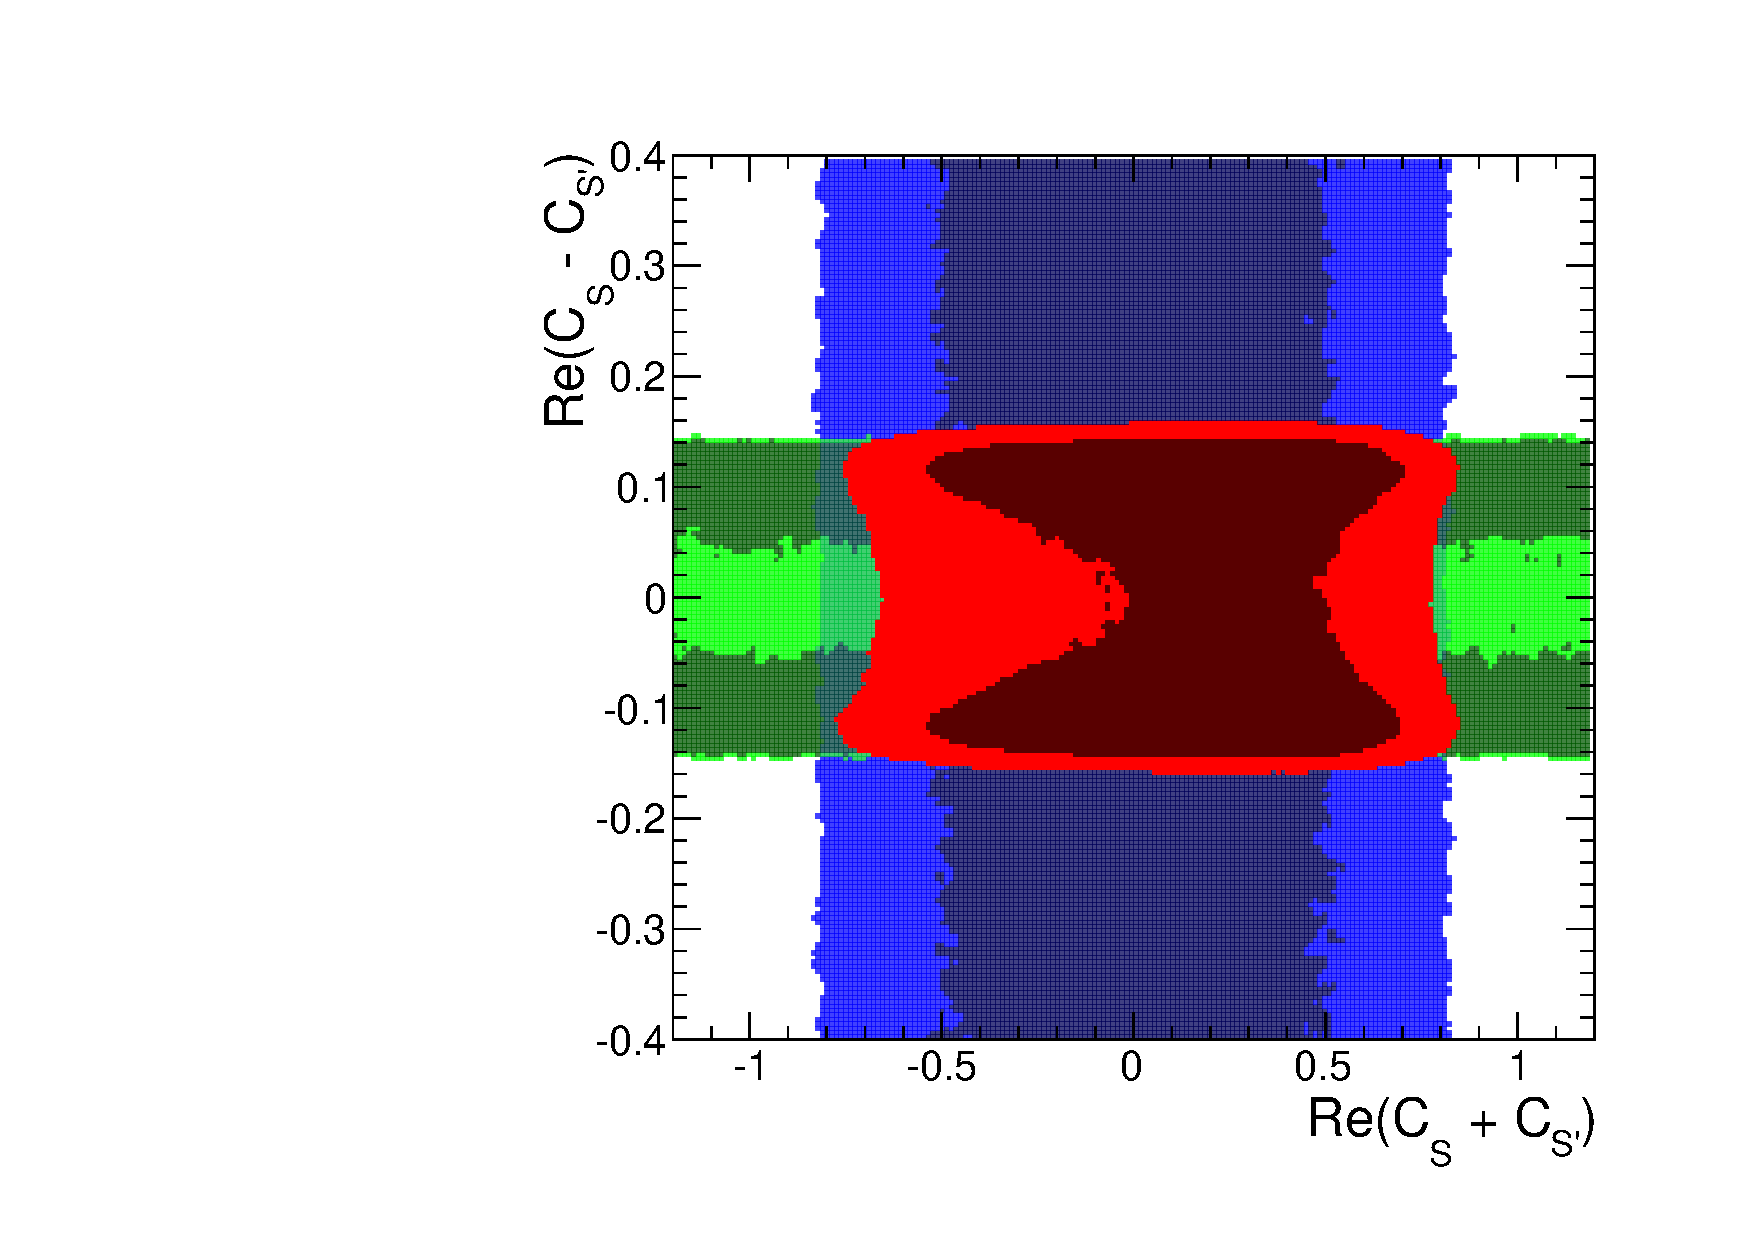
\includegraphics[width=.325\textwidth]{plots/pdf/res-SSp.pdf}
%  \includegraphics[width=.32\textwidth]{plots/pdf/res-PPp.pdf}
  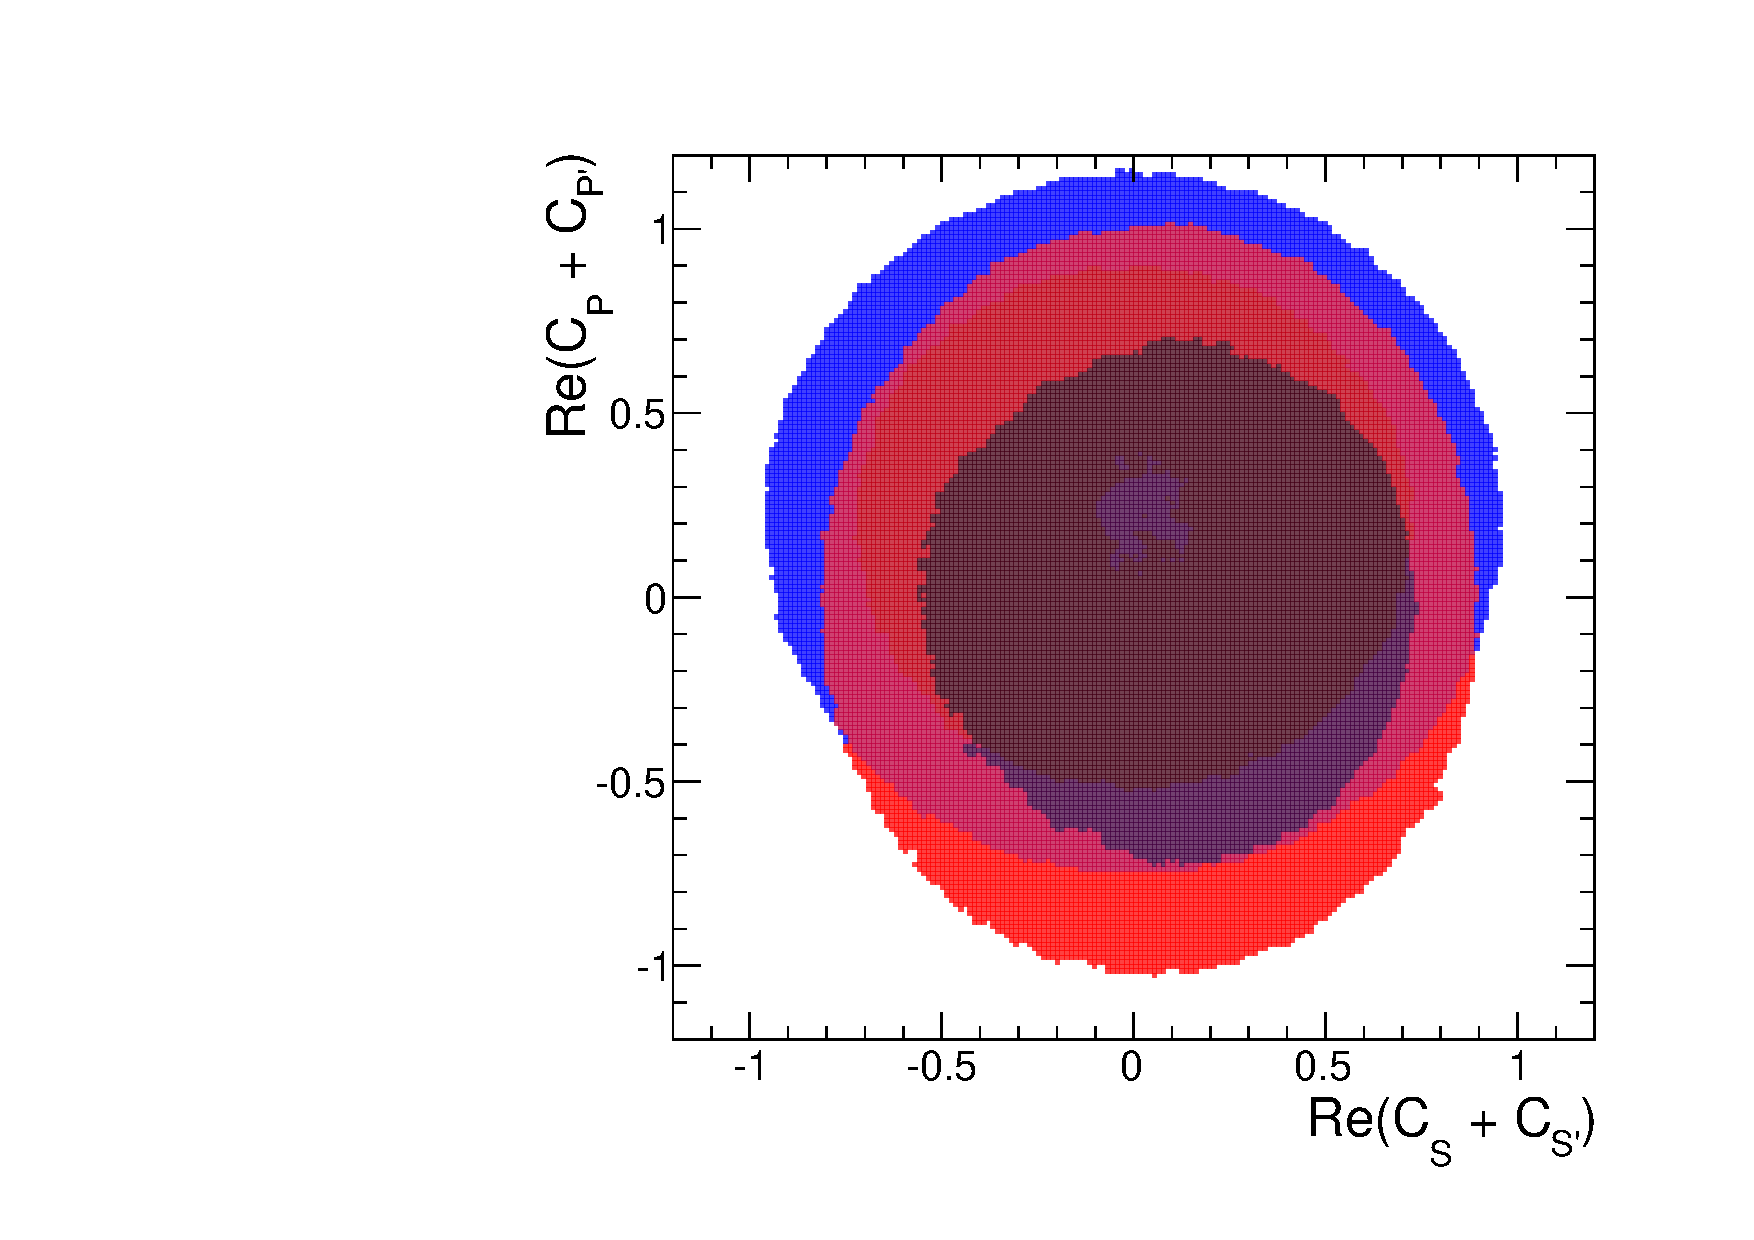
\includegraphics[width=.325\textwidth]{plots/pdf/res-SPplus.pdf}
  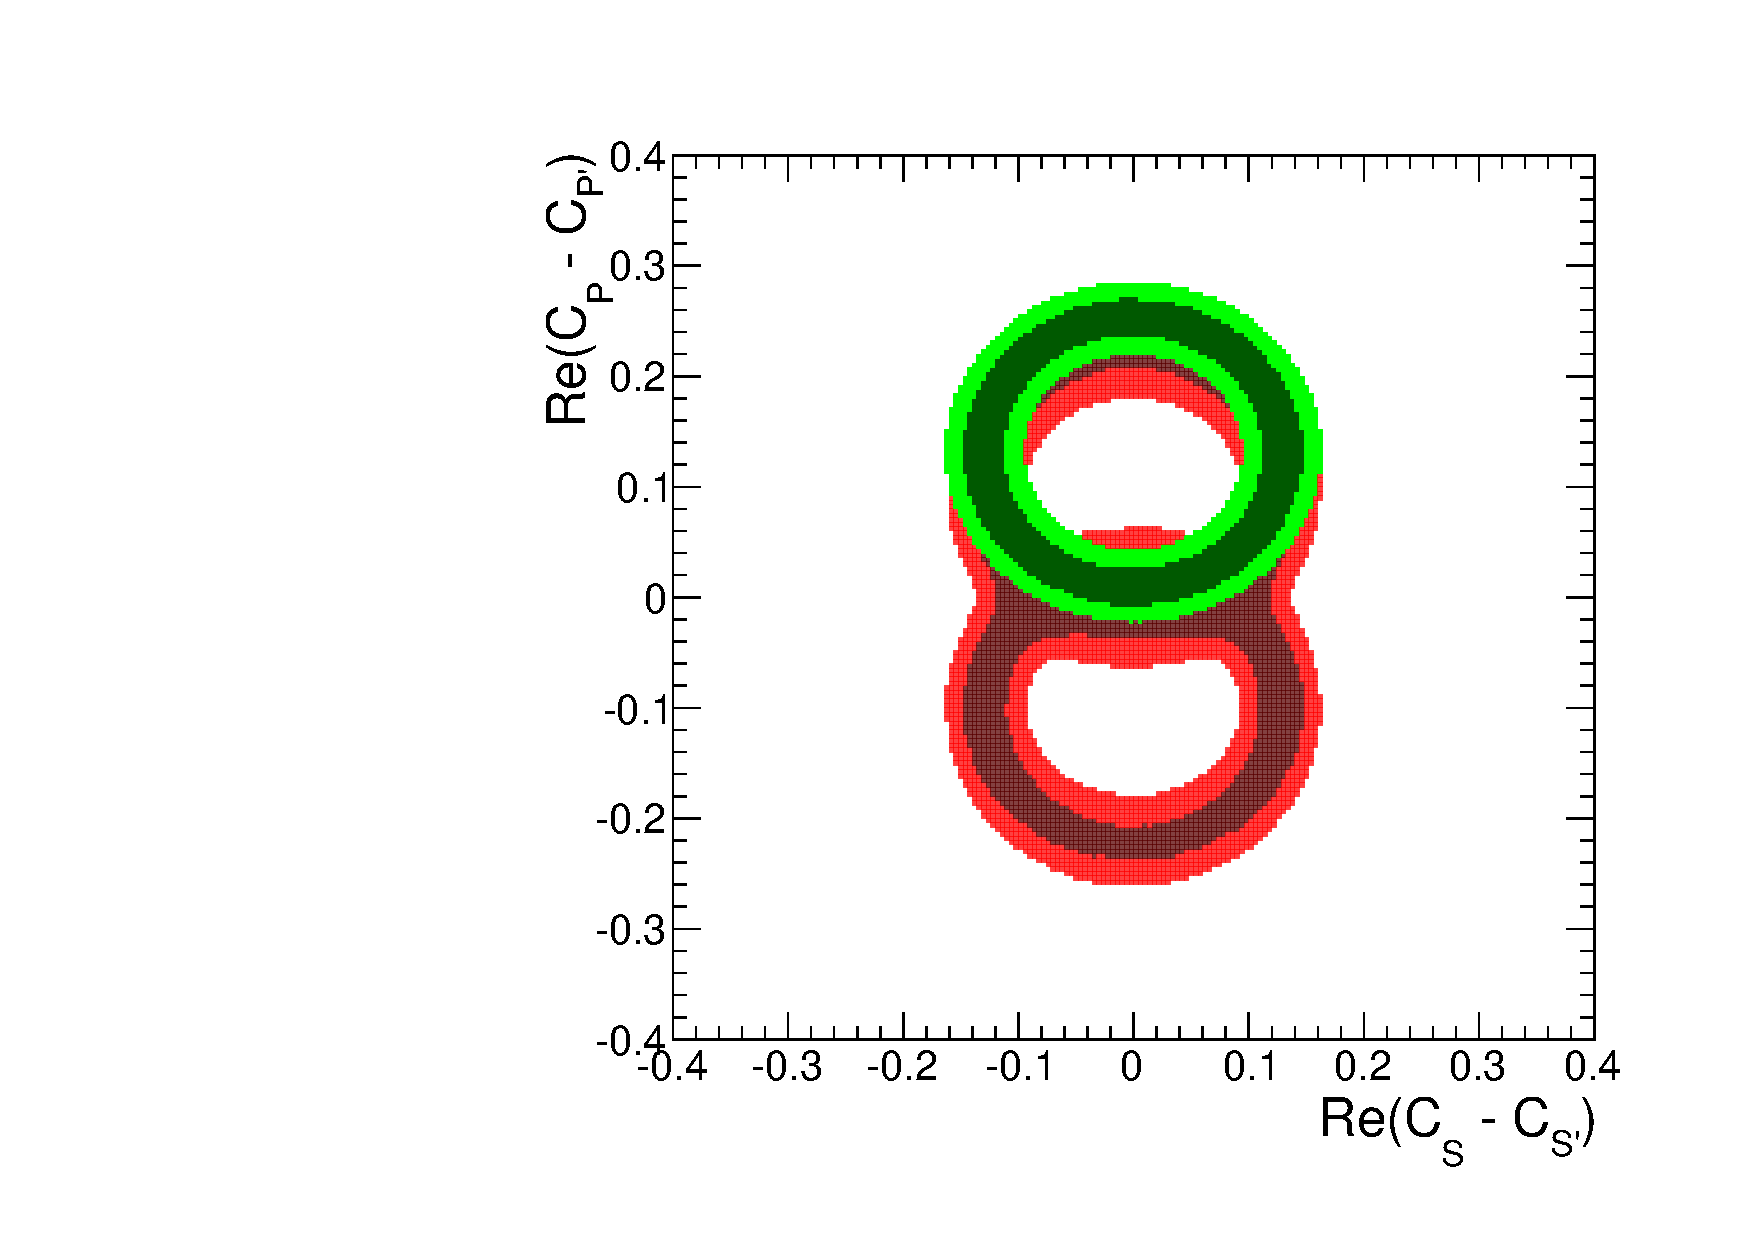
\includegraphics[width=.325\textwidth]{plots/pdf/res-SPminus.pdf}
  \caption{
    \eos{
    Constraints on real-valued scalar couplings $\wilson{S,\,S',\,P,\,P'}$ 
    from only $F_H^\mu$~(blue), only $\overline{\cal B}(B_s \to \bar\mu\mu)$ (green) 
    and their combination with other data in \reftab{tab:observables} as well as
    $\wilson[NP]{10} \in [-1,\, 9]$, $\wilson[NP]{10'} \in [-5,\,5]$ (red) 
    at 68\% (darker) and 95\% (lighter) probability. The constraints on 
    $(\wilson{P}�\pm \wilson{P'})$ are identical to $(\wilson{S}�\pm \wilson{S'})$
    [left], apart from a small shift of the contours by $(+0.2,\, 0.15)$.
    }
  }
  \label{fig:scalar}
\end{figure*}

Interference terms of $\wilson{P,\,P'}$ with vectorial couplings might weaken 
bounds. Most important for $\overline{\cal B}(B_s \to \bar\mu\mu)$ are 
$(\wilson{10} - \wilson{10'})$ --- compare \refeq{eq:Br-Bsmumu:time0} --- and
for $F_H^\ell$ similarly $(\wilson{10} + \wilson{10'})$ \cite{Bobeth:2007dw},
which are suppressed by factors $m_\ell/M_{B_s}$ and $m_\ell/\sqrt{q^2}$,
respectively. However, due to the large SM contribution of $\wilson[SM]{10}
\simeq -4.2$, these terms are important for small pseudo-scalar couplings.
We compile constraints on complex-valued scalar couplings from $i)$ only
$F_H^\mu$, $ii)$ only $\overline{\cal B}(B_s \to \bar\mu\mu)$ and $iii)$
their combination, even allowing new physics in $\wilson{10,\, 10'}$ in
\reftab{tab:cSP:1-dimCLs}. Neither $F_H^\ell$ nor $\overline{\cal B}(B_s \to \bar\mu\mu)$
alone can bound all four complex-valued scalar couplings, however their
combination is capable to do so and moreover, the bounds are stable against
destructive interference with vectorial couplings. In the general case
of complex-valued couplings, $\overline{\cal B}(B_s \to \bar\mu\mu)$ does
not provide anymore constraints on sub-intervals in contrast to the
case of real-valued couplings. In consequence, for example the ring-like
structure in the $(\wilson{S}-\wilson{S'}) - (\wilson{P}-\wilson{P'}) $-plane
of \reffig{fig:scalar} would turn into a filled circle.

Our results improve and extend previous constraints in the literature to
the most general case of complex-valued couplings. For example they are
a factor \eos{two to three} more stringent then \cite{Becirevic:2012fy} and
\eos{comparable} to \cite{Altmannshofer:2012az} once restricting to scenarios
considered there.

\begin{table*}
  \renewcommand{\arraystretch}{1.3}
  %\resizebox{\textwidth}{!}{
  \begin{tabular}{c|ccc}
  \hline
  data set
  & only $F_H^\mu$
  & only $\overline{\cal B}(B_s \to \bar\mu\mu)$
  & all
  \\ 
  set of couplings
  & $\wilson{S,\,S',\,P,\,P'}$
  & $\wilson{S,\,S',\,P,\,P'}$
  & $\wilson{S,\,S',\,P,\,P'\,10,\,10'}$
  \\
  \hline \hline
  $\mbox{Re}(\wilson{S} - \wilson{S'})$
  & $\quad$ $-$ $\quad$
  & \eos{$\quad$ $[-0.08,\, 0.08]$ ($[-0.12,\, 0.12]$) $\quad$}
  & \eos{$\quad$ $[-0.08,\, 0.08]$ ($[-0.12,\, 0.12]$) $\quad$}
  \\
  $\mbox{Im}(\wilson{S} - \wilson{S'})$
  & $\quad$ $-$ $\quad$
  & \eos{$\quad$ $[-0.08,\, 0.08]$ ($[-0.12,\, 0.12]$) $\quad$}
  & \eos{$\quad$ $[-0.08,\, 0.08]$ ($[-0.12,\, 0.12]$) $\quad$}
  \\[0.1cm]
  $\mbox{Re}(\wilson{S} + \wilson{S'})$
  & \eos{$[-0.4,\, 0.4]$ ($[-0.7,\, 0.7]$)}
  & $-$
  & \eos{$[-0.3,\, 0.4]$ ($[-0.6,\, 0.7]$)}
  \\
  $\mbox{Im}(\wilson{S} + \wilson{S'})$
  & \eos{$[-0.4,\, 0.4]$ ($[-0.7,\, 0.7]$)}
  & $-$
  & \eos{$[-0.4,\, 0.4]$ ($[-0.7,\, 0.7]$)}
  \\[0.1cm]
  $\mbox{Re}(\wilson{P} - \wilson{P'})$
  & $-$
  & \eos{$[0.06,\, 0.20]$  ($[0.02,\, 0.25]$)}
  & \eos{$[-0.10,\, 0.10]$ ($[-0.18,\, 0.18]$)}
  \\
  $\mbox{Im}(\wilson{P} - \wilson{P'})$
  & $-$
  & \eos{$[-0.08,\, 0.08]$ ($[-0.12,\, 0.12]$)}
  & \eos{$[-0.10,\, 0.10]$ ($[-0.20,\, 0.20]$)}
  \\[0.1cm]
  $\mbox{Re}(\wilson{P} + \wilson{P'})$
  & \eos{$[-0.2,\, 0.6]$ ($[-0.5,\, 0.9]$)}
  & $-$
  & \eos{$[-0.4,\, 0.4]$ ($[-0.7,\, 0.7]$)}
  \\
  $\mbox{Im}(\wilson{P} + \wilson{P'})$
  & \eos{$[-0.4,\, 0.4]$ ($[-0.7,\, 0.7]$)}
  & $-$
  & \eos{$[-0.4,\, 0.4]$ ($[-0.7,\, 0.7]$)}
  \\
  \hline 
  \end{tabular}
%}
  \renewcommand{\arraystretch}{1.0}
  \caption{
     \label{tab:cSP:1-dimCLs}
     The constraints on complex-valued $\wilson{S,\,S',\,P,\,P'}$ --- 1D-marginalized 
     at 65\% (95\%) probability --- when using measurements of $i)$ only $F_H^\mu$,
     $ii)$ only $\overline{\cal B}(B_s \to \bar\mu\mu)$ and $iii)$ all the data in
     \reftab{tab:observables} allowing also for new physics contributions to 
     $\wilson{10,\,10'}$ with \eos{uniform prior $\mbox{Re}\,\wilson[NP]{10} \in [-1,\, 9]$,
     $\mbox{Im}\,(\wilson[NP]{10})$ and $\mbox{Re},\mbox{Im}\,(\wilson[NP]{10'}) \in [-5,\, 5]$}.
  }
\end{table*}

%
%
%--------+---------+---------+---------+---------+---------+---------+---------+
\subsection{SM-EFT-constrained scalar couplings}

In the following we consider a model-independent scenario as predicted by the SM
augmented by dimension six operators that respect the SM gauge group and are
composed out of SM fields. After the discovery of a scalar resonance at the LHC
that complies currently with all requirements of the Higgs particle in the SM
and the steadily rising lower bounds on new particle masses towards higher energies 
from ATLAS and CMS such a scenario becomes more and more viable. 

A non-redundant set of dimension six operators of
this effective theory (SM-EFT) was given in \cite{Grzadkowski:2010es} and the
matching to the effective theory of $\Delta B = 1$ decays \refeq{eq:Heff} at the
scale $\mu \sim m_W$ of the order of the $W$-boson mass in \cite{D'Ambrosio:2002ex}
for vectorial couplings $\wilson{7,\,9,\,10}$. The matching for tensor
\refeq{eq:tensor:ops} and scalar \refeq{eq:scalar:ops} operators 
\cite{Alonso:2014csa} shows that SM gauge groups impose the relations
\begin{align}
  \wilson{P}  & = -\wilson{S}\,, &
  \wilson{P'} & = \wilson{S'}\,, &
  \wilson{T}  & = \wilson{T5} = 0
\end{align}
on scalar and pseudo-scalar couplings and require tensorial couplings to be
suppressed to the level of dimension eight operators. In consequence only two
scalar couplings $\wilson{S,\, S'}$ arise that scale as $\sim v^2/\Lambda_{\rm NP} \ll 1$
where $v^2$ denotes the scale of electroweak symmetry breaking and $\Lambda_{\rm NP}$
a high energy scale at which new physics generates these operators.

The couplings $\wilson{S,\, S'}$ can be bound quite reliably from (neglecting
terms of order $m_\ell^2/M_{B_s}^2$ and $m_s/m_b$) \cite{Alonso:2014csa}
\begin{equation}
\begin{aligned}
  \overline{\cal B}(B_s\to \bar\ell\ell) & \propto
      \left|\wilson{S} + \wilson{S'}\right|^2
    + \left|\wilson{S} - \wilson{S'}\right|^2 
\\[0.2cm]
  - & \frac{4 m_\ell\, m_b}{M_{B_s}^2} \mbox{Re} 
  \left[ (\wilson{S} + \wilson{S'})(\wilson{10} - \wilson{10'})^* \right]
\end{aligned}
\end{equation}
and almost similarly (neglecting terms of order $m_\ell^2/q^2$
and $m_s/m_b$)
\begin{equation}
\begin{aligned}
  F_H^\ell & \propto
      \left|\wilson{S} + \wilson{S'}\right|^2
    + \left|\wilson{S} - \wilson{S'}\right|^2 
\\[0.2cm] 
  & - \frac{4 m_\ell\, m_b}{q^2} \mbox{Re} 
  \left[ (\wilson{S} - \wilson{S'})(\wilson{10} + \wilson{10'})^* \right] \,.
\end{aligned}
\end{equation}

The SM gauge groups do not impose constraints on the operators of the SM-EFT that
imply relations among $\wilson{10}$ and $\wilson{10'}$, so they
are in general additional independent parameters. Here we find that destructive
interference with contributions involving $\wilson{10,\, 10'}$ do not change
much upper bounds on $|\wilson{S,\, S'}|$ found in \cite{Alonso:2014csa}. However,
for the most general case of complex-valued couplings destructive interference
constrains (4 parameters) \todo{finish, describe \reffig{fig:scalar:SM-EFT}}

\begin{figure*}
  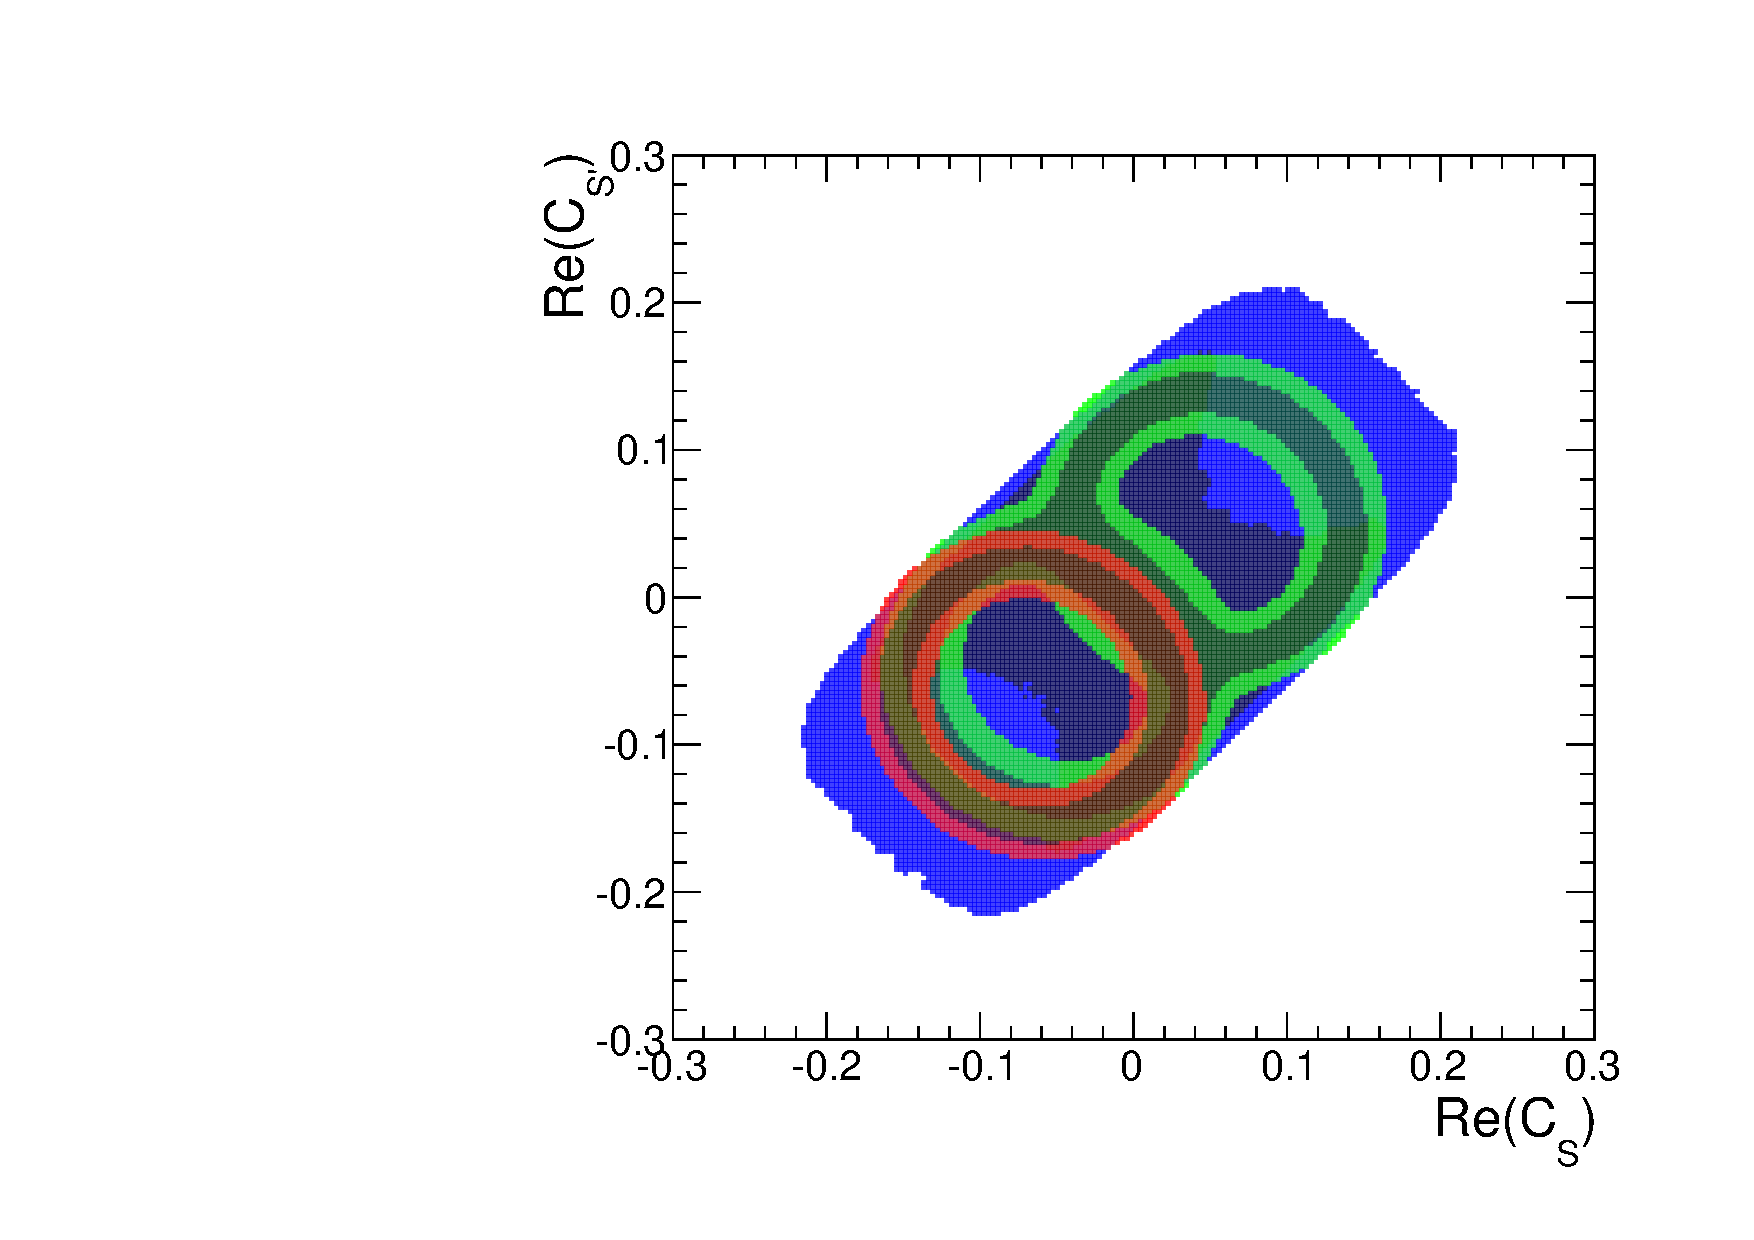
\includegraphics[width=.35\textwidth]{plots/pdf/res-real_SSp_constr.pdf}
  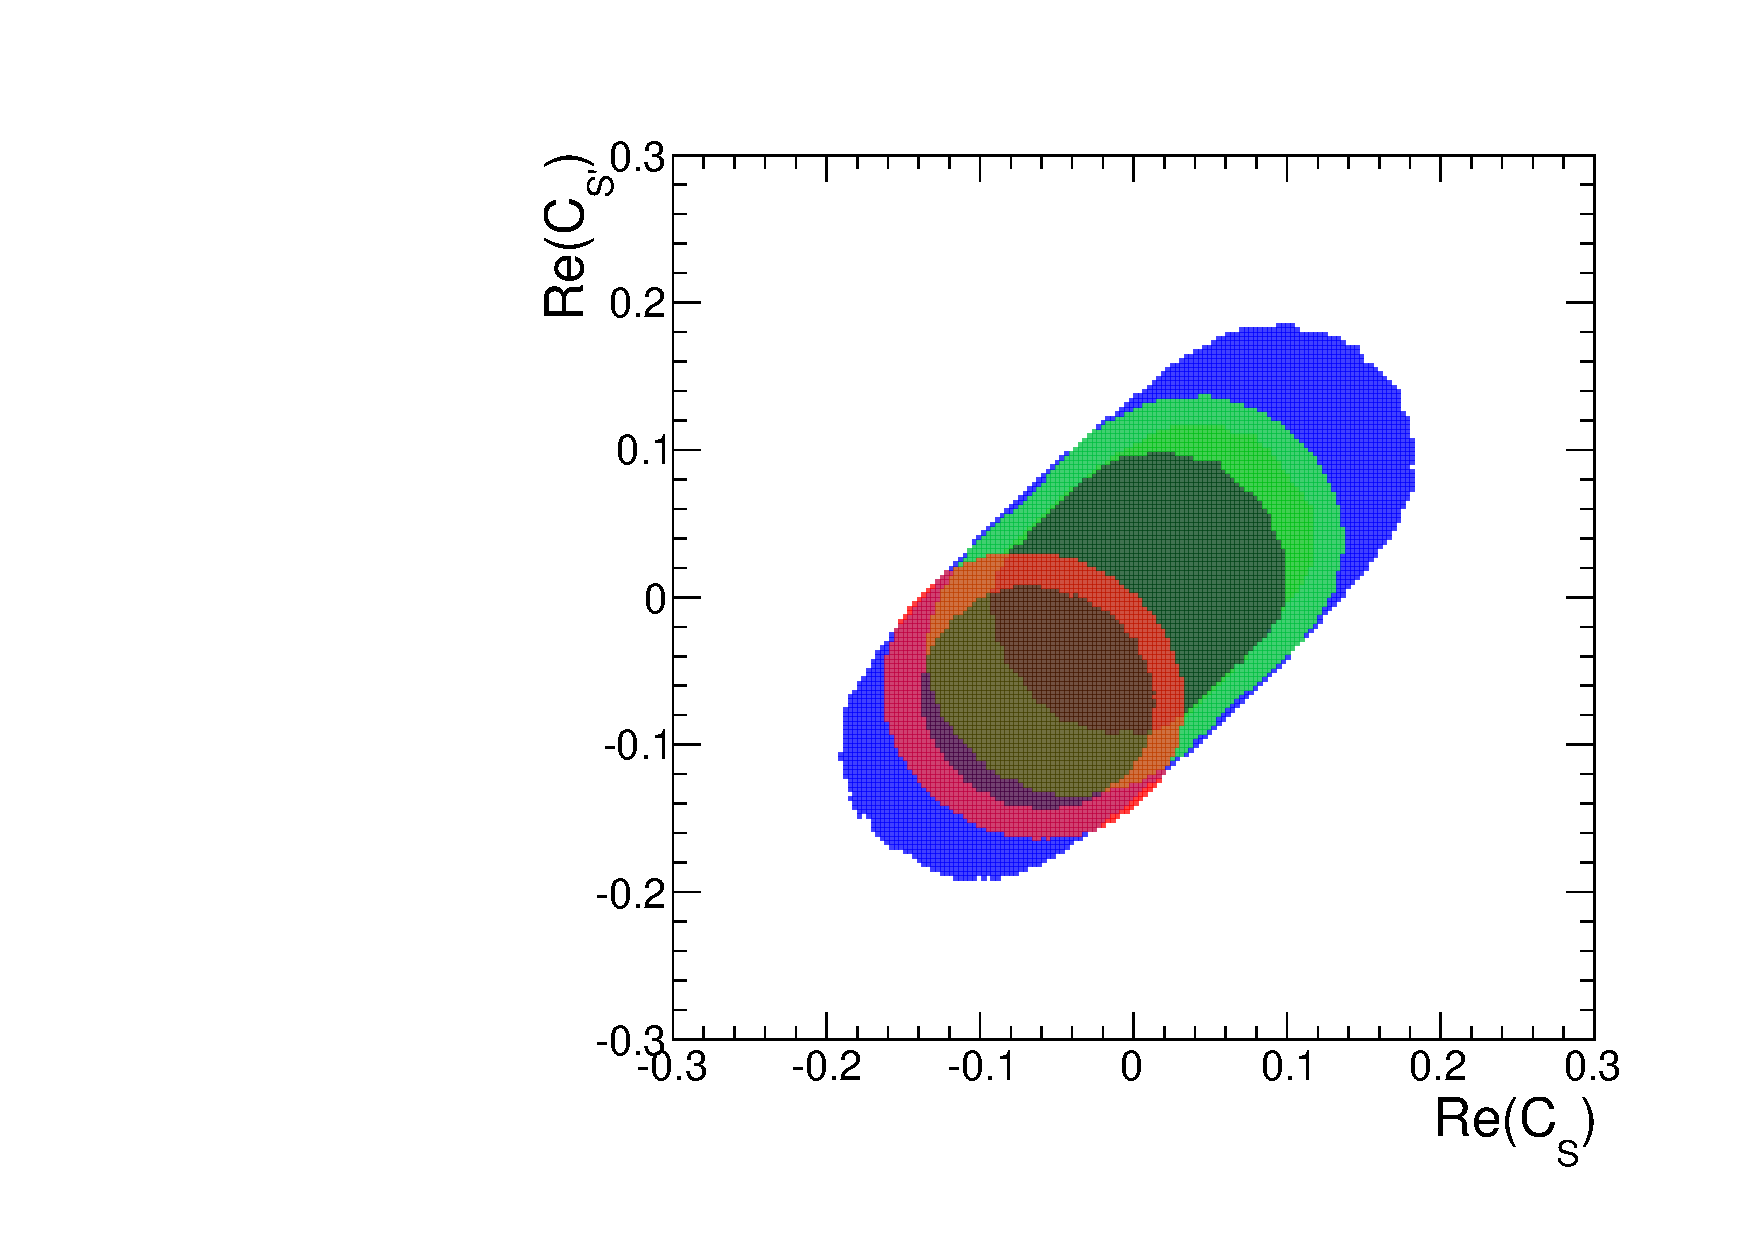
\includegraphics[width=.35\textwidth]{plots/pdf/res-cmplx_SSp_constr.pdf}
  \caption{
    \eos{
    Constraints on real-valued [left] and complex-valued [right] scalar couplings 
    $\wilson{S,\,S'}$ in the scenario SM-EFT from only $\overline{\cal B}(B_s \to 
    \bar\mu\mu)$ (blue) and all data in \reftab{tab:observables} (green) 
    at 68\% (darker) and 95\% (lighter) probability when marginalising
    over non-zero $\mbox{Re}(\wilson[NP]{10}) \in [-1,\, 9]$ as well as and 
    $\mbox{Im}(\wilson[NP]{10})$ and $\mbox{Re, Im}(\wilson[NP]{10'}) \in [-5,\,5]$.
    For comparison the according constraints from all data when keeping
    $\mbox{Re, Im}(\wilson[NP]{10,\, 10'}) = 0$ (red)
    at 68\% (darker) and 95\% (lighter) probability. 
    }
  }
  \label{fig:scalar:SM-EFT}
\end{figure*}

%
%
%--------+---------+---------+---------+---------+---------+---------+---------+
\subsection{Tensorial, scalar and vectorial couplings and
  predictions for $B\to K^* \bar\ell\ell$}

We start with the scenario of the combination of tensorial and scalar couplings
$\wilson{S,S',P,P',T,T5}$, i.e. the combination of the preceding
two sections. In this scenario there are only small changes on the bounds, in fact
they tend to be even more stringent, because tensorial and scalar couplings
can contribute to $F_H^{\mu}$ only constructively --- see \refeq{eq:FH-dependence}.
As before ${\cal B}$'s of $B\to K^{(*)}\bar\mu\mu$ help to strengthen the
constraints on $\wilson{T,\, T5}$. Furthermore we find that even in the case
of complex-valued couplings the data is able to constrain all real and imaginary
parts. In this case, the constraints are even a bit tighter and strong correlations
arise as before among real parts of $\wilson{i}$ and $\wilson{i'}$ for $i = S,P$,
and in addition similarly among their imaginary parts.  
\todo{Check this with EOS}

In the remainder we discuss the influence of non-standard $\wilson{10,\, 10'}$,
that play an important role in $\overline{\cal B}(B_s \to \bar\mu\mu)$ ...

\begin{table*}
  \renewcommand{\arraystretch}{1.3}
  %\resizebox{\textwidth}{!}{
  \begin{tabular}{cc|cc}
  \hline
    observable
  & $q^2$-bin [GeV$^2$]
  & SM
  & NP
  \\
  \hline \hline
  \multirow{2}{*}{$J_{6c}$}
  & $[1.1,\, 6]$
  & $[ ,\, ]$ ($[ ,\, ]$)
  & $[ ,\, ]$ ($[ ,\, ]$)
  \\
  & $[15,\, 19]$
  & $[ ,\, ]$ ($[ ,\, ]$)
  & $[ ,\, ]$ ($[ ,\, ]$)
  \\
  \hline
  \multirow{2}{*}{$J_{1c} + J_{2c}$}
  & $[1.1,\, 6]$
  & $[ ,\, ]$ ($[ ,\, ]$)
  & $[ ,\, ]$ ($[ ,\, ]$)
  \\
  & $[15,\, 19]$
  & $[ ,\, ]$ ($[ ,\, ]$) 
  & $[ ,\, ]$ ($[ ,\, ]$)
  \\
  \hline
  \multirow{2}{*}{$J_{1s} - 3 J_{2s}$}
  & $[1.1,\, 6]$
  & $[ ,\, ]$ ($[ ,\, ]$)
  & $[ ,\, ]$ ($[ ,\, ]$)
  \\
  & $[15,\, 19]$
  & $[ ,\, ]$ ($[ ,\, ]$) 
  & $[ ,\, ]$ ($[ ,\, ]$)
  \\
  \hline 
  \end{tabular}
%}
  \renewcommand{\arraystretch}{1.0}
  \caption{
     \label{tab:predictions}
     \todo{predictions for $B\to K^*\bar\ell\ell$}
  }
\end{table*}

%
%
%
%--------+---------+---------+---------+---------+---------+---------+---------+
\section{Conclusions}

We have derived to date most stringent constraints on tensorial and scalar
couplings that mediate $b\to s\bar\mu\mu$ utilising the latest measurements
of angular observables $F_H^\mu$ and the lepton forward-backward asymmetry
$A_{\rm FB}^\mu$ in $B^+\to K^+ \bar\mu\mu$ from LHCb \cite{Aaij:2014tfa},
supplemented by measurements of the branching ratios of $B_s\to \bar\mu\mu$ and
$B\to K^{(*)} \bar\mu\mu$. Both observables, $F_H^\mu$ and $A_{\rm FB}^\mu$,
belong to a class in which vectorial and dipole couplings that arise also in
the standard model (SM) are suppressed (mostly kinematically by $m_\ell / 
\sqrt{q^2}$) w.r.t tensorial and scalar couplings. We provide predictions for
analogous but not yet measured angular observables $J_{6c}$, $(J_{1c} + J_{2c})$
and $(J_{1s} - 3 J_{2s})$ in $B\to K^* (\to K\pi) \bar\mu\mu$ .

We find that the experimental measurement of $F_H^\mu$
\begin{enumerate}
\item imposes by itself constraints on tensorial couplings \eos{$|{\cal C}_{T,\,T5}^\mu|
  < 0.35\, (0.55)$} at 68\% (95\%) probability, superseding previous bounds.
  In combination with current data from $B\to K^* \bar\mu\mu$ and lattice
  $B\to K^*$ form factors they become tighter \eos{$|{\cal C}_{T,\,T5}^\mu| < 0.30\, 
  (0.45)$}, even in the presence of non-standard contributions in vectorial
  couplings.
\item allows for the first time to bound all four scalar and pseudo-scalar 
  couplings due to it's complementarity to $\overline{\cal B}(B_s \to \bar\mu\mu)$.
  Even when taking into account destructive interference with vectorial couplings
  \eos{$|\wilson{i} + \wilson{i'}| < 0.4\, (0.7)$ and $|\wilson{i} - \wilson{i'}| < 
  0.1\, (0.2)$} for $i = S,P$ at 68\% (95\%) probability. Currently, the bounds 
  from $F_H^\mu$ are not as strong as those from $\overline{\cal B}(B_s \to \bar\mu\mu)$
  by a factor four. In the future, measurements at LHCb and Belle II will 
  further tighten the bounds. Moreover, measurements of $F_H^e$ ($\ell = e$)
  will provide constraints on scalar couplings in the electron channel in
  the lack of measurements of $B_s \to \bar{e}e$. 
\item SM-EFT $\ldots$
\end{enumerate}
In all cases these \eos{constraints are weakened only slightly} in the presence of
new physics in vectorial couplings from destructive interference. 


%
%
%
%--------+---------+---------+---------+---------+---------+---------+---------+
\begin{acknowledgments}
  We are grateful to Danny van Dyk for helpful discussions and his support on
  EOS \cite{EOS} and Chris Bouchard for communications concerning $B\to K$
  form factors \cite{Bouchard:2013eph}.
  C.B. received partial support from the ERC Advanced Grant project ``FLAVOUR'' 
  (267104).
\end{acknowledgments}


%--------+---------+---------+---------+---------+---------+---------+---------+
%
%  Appendix
%
%--------+---------+---------+---------+---------+---------+---------+---------+

\appendix

%
%
%
%--------+---------+---------+---------+---------+---------+---------+---------+
\section{
  Angular observables in $B\to K^* \bar\ell\ell$
  \label{app:BKstarellell}
}

Here we present those angular observables $J_i$ in $B\to K^* \bar\ell\ell$
in which tensorial and scalar contributions are kinematically enhanced by a factor
$\sqrt{q^2}/m_\ell$ over vectorial once present in the SM or their respective 
interference terms using results and notation from \cite{Bobeth:2012vn}. 

For convenience, we split the time-like transversity amplitude into
\begin{align}
  A_t & 
  = \tilde{A}_t - \frac{1}{2} \frac{\sqrt{q^2}}{m_\ell} A_P
\end{align}
that depend on the Wilson coefficients $i = 10, 10', P, P'$ and the scalar
$B\to K^*$ form factor $A_0(q^2)$, a normalisation factor $N$ and the 
K{\"a}ll{\'e}n-function $\lambda$ (see \cite{Bobeth:2012vn})
\begin{equation}
\begin{aligned}
  \tilde{A}_t & = 2 N \frac{\sqrt{\lambda}}{\sqrt{q^2}}
    (\wilson[]{10} - \wilson[]{10'}) A_0\,,
\\
  A_P & = - 2 N\sqrt{\lambda} \frac{(\wilson[]{P} - \wilson[]{P'})}{(m_b+m_s)} A_0\,.
\end{aligned}
\end{equation}
The lepton-flavor index $\ell$ at Wilson coefficients is omitted for
brevity throughout this section.

In full generality angular observables in $B\to K^* \bar\ell\ell$ depend on
seven transversity amplitudes with vectorial and dipole contributions 
$A_{0,\,\perp,\,\parallel}^{L,R}$, and $\tilde{A}_t$, one scalar and one
pseudoscalar amplitude $A_{S,\,P} \propto (\wilson[]{S,P} - \wilson[]{S',P'})$, 
and six tensorial amplitudes: $A_{\parallel\perp,\,t\perp,\,0\parallel} \propto 
\wilson[]{T}$ and $A_{t0,\,t\parallel,\,0\perp} \propto \wilson[]{T5}$. 
The interesting combinations are

\begin{widetext}
\begin{align}
  \frac{4}{3} J_{6c} & =
  4\, \beta_\ell\, \mbox{Re} \bigg[ 2\, (A_{t0}^{} A_S^* - A_{\parallel\perp}^{} A_P^*) + 
      \frac{m_\ell}{\sqrt{q^2}} \big[(A_0^L + A_0^R) A_S^* 
           + 4\, A_{\parallel\perp}^{} \tilde{A}_t^* \big] \bigg],
\\
  \frac{4}{3}\(J_{1c} + J_{2c}\) & =
    \Bigg| \frac{2\, m_\ell}{\sqrt{q^2}} (A_0^L + A_0^R) + 4\, A_{t0} \Bigg|^2
   + \Bigg|\frac{2\, m_\ell}{\sqrt{q^2}}\, \tilde{A}_t - A_P\Bigg|^2 + \beta_\ell^2\, |A_S|^2
   + 16\, \beta_\ell^2\, |A_{\parallel\perp}|^2,
\\[0.2cm]
  \frac{4}{3}\(J_{1s} - 3\, J_{2s}\) &  =
    \Bigg| \frac{\sqrt{2}\, m_\ell}{\sqrt{q^2}} (A_\perp^L + A_\perp^R) + 4\, A_{t\perp} \Bigg|^2
  + \Bigg| \frac{\sqrt{2}\, m_\ell}{\sqrt{q^2}} (A_\parallel^L + A_\parallel^R) + 4\, A_{t\parallel} \Bigg|^2.
\end{align}
\end{widetext}
Above $\beta_\ell^2 = 1 - 4 m_\ell^2/q^2 \to 1$ for $m_\ell \ll \sqrt{q^2}$.
The condition is well fulfilled for $\ell = e$ and $1\, \mbox{GeV}^2\lesssim q^2$,
provided that tensorial and scalar Wilson coefficients do not receive additional 
suppression factors. For $\ell = \mu$ the value of $q^2$ should not be too low,
whereas in the case $\ell = \tau$, these observables are not anymore dominated by 
tensorial and/or scalar contributions alone, and the full lepton-mass dependence has
to be taken into account. 

Finally, we note that the term
\begin{widetext}
\begin{align}
  \Bigg|\frac{2\, m_\ell}{\sqrt{q^2}}\, \tilde{A}_t - A_P\Bigg|^2
  + \beta_\ell^2\, |A_S|^2  & = 
  4 N^2 \lambda A_0^2 \Bigg\{ 
    \beta_\ell^2 \Bigg|\frac{\wilson[]{S} - \wilson[']{S}}{m_b + m_s}\Bigg|^2 
  + \Bigg|\frac{\wilson[]{P} - \wilson[']{P}}{m_b + m_s}
     + \frac{2 m_\ell}{q^2} \big(\wilson[]{10} - \wilson[']{10}\big) \Bigg|^2 
    \Bigg\}
\end{align}
entering $(J_{1c} + J_{2c})$, resembles very much the branching ratio of the rare
decays $B_s \to \bar\ell\ell$ in the limit $q^2 \to M_{B_s}^2$
\begin{equation}
\label{eq:Br-Bsmumu:time0}
\begin{aligned}
  {\cal B}(B_s \to \bar\ell\ell) & = 
    \frac{G_F^2 \alpha_e^2 |V_{tb}^{} V_{ts}^*|^2}{64\, \pi^3} 
    M_{B_s}^5 f_{B_s}^2 \tau_{B_s} \beta_\ell(q^2 = M_{B_s}^2) 
\\
   & \hskip0.5cm \times \Bigg\{ 
    \beta_\ell^2(q^2 = M_{B_s}^2) \Bigg|\frac{\wilson[]{S} - \wilson[']{S}}{m_b + m_s}\Bigg|^2 
  + \Bigg|\frac{\wilson[]{P} - \wilson[']{P}}{m_b + m_s}
     + \frac{2 m_\ell}{M_{B_s}^2} \big(\wilson[]{10} - \wilson[']{10}\big) \Bigg|^2 
    \Bigg\}\,.
\end{aligned}
\end{equation}
\end{widetext}
Hence there is some complementarity among $(J_{1c} + J_{2c})$ in $B \to K^*
\bar\ell\ell$ and ${\cal B}(B_s \to \bar\ell\ell)$, however former depends also
on tensorial couplings and vectorial couplings. The helicity suppression
factor $4\,m_\ell^2/q^2$ of vector couplings is weaker in 
$B \to K^* \bar\ell\ell$ decays than the corresponding factor 
$4\,m_\ell^2/M_{B_s}^2$ in $B_s \to \bar\ell\ell$.

Concerning $B_s\to \bar\ell\ell$, the expression \refeq{eq:Br-Bsmumu:time0} 
corresponds to the unintegrated branching ratio at time $t=0$. Due to the non-vanishing
decay width $\Delta\Gamma_s$, experiments measure the average 
time-integrated branching ratio --- denoted by $\overline{\cal B}$ --- 
and both are related as \cite{DeBruyn:2012wk} 
\begin{align}
  \label{eq:Br-Bsmumu}
  \overline{\cal B} (B_s \to \bar\ell\ell) & 
  = \frac{1 + y_s {\cal A}_{\Delta\Gamma}}{1 - y_s^2} {\cal B} (B_s \to \bar\ell\ell)\,.
\end{align}
Here $y_s \equiv \Delta\Gamma_s/(2\Gamma_s)$ with the numerical value given in
\cite{Beaujean:2013soa}. ${\cal A}_{\Delta\Gamma}$ is the CP asymmetry
due to nonvanishing width difference, which is ${\cal A}_{\Delta\Gamma} = 1$
in the SM, but in general can be ${\cal A}_{\Delta\Gamma} \in [-1,\, 1]$. 
Since ${\cal A}_{\Delta\Gamma}$ can depart from it's SM value in scenarios of
new physics considered in this work, we take this effect into account
in our numerical analysis, although it is suppressed by small $y_s$. The latest
SM prediction $\overline{\cal B} (B_s \to \bar\mu\mu) = (3.65 \pm 0.23) \cdot 
10^{-9}$~\cite{Bobeth:2013uxa} includes NLO electroweak \cite{Bobeth:2013tba} 
and NNLO QCD corrections \cite{Hermann:2013kca}.

Finally we discuss the possibility of suitable normalisations of $J_{6c}$,  
$(J_{1s} - 3\, J_{2s})$ and $(J_{1c} + J_{2c})$ at high $q^2$ that would provide
optimised observables. For this purpose we use form factor relations at leading
order in $1/m_b$ and neglect terms suppressed by $m_\ell/\sqrt{q^2}$. With the
notation and expressions derived in \cite{Bobeth:2012vn},
\begin{equation}
\begin{aligned}
  J_{1s} - 3\, J_{2s} & = \frac{3}{2}\, \rho_1^T (f_\perp^2 + f_\parallel^2) \,,
\\[0.1cm]
  J_{1c} + J_{2c} & = 3\, \rho_1^T f_0^2 
     + \frac{3 N^2 \lambda}{(m_b+m_s)^2} A_0^2
\\ 
   & \quad \times \left(|\wilson{S}-\wilson{S'}|^2 + |\wilson{P}-\wilson{P'}|^2\right)\,.
\\[0.1cm]
  \frac{4}{3} J_{6c} & = \todo{???}
\end{aligned}
\end{equation}
Here $f_{\perp, \parallel, 0}$ and $A_0$ denote $B\to K^*$ form factors, whereas
the $\rho_1^\pm$ depends on vectorial couplings and $\rho_1^T \propto 
(|\wilson{T}|^2 + |\wilson{T5}|^2)$.

Concerning $(J_{1s} - 3\, J_{2s})$, there are no appropriate normalisations,
unless chirality-flipped $\wilson[NP]{7',\,9',\,10'} = 0$ vanish, because then
$\rho_1^+ = \rho_1^-$ holds. There are three potential normalisations
\begin{equation}
\begin{aligned}
  \frac{4}{3} & J_{1s} =
    (3 \rho_1^+ + \rho_1^T) f_\perp^2 +  (3 \rho_1^- + \rho_1^T) f_\parallel^2 \,,
\\
  \frac{8}{3} & J_{2s} =
    (\rho_1^+ - \rho_1^T) f_\perp^2 +
    (\rho_1^- - \rho_1^T) f_\parallel^2 \,,
\\[0.1cm]
  & J_{1s} + 2 J_{2s} =
    3 (\rho_1^+ f_\perp^2 + \rho_1^- f_\parallel^2) \,
\end{aligned}
\end{equation}
where the last one depends only on vectorial couplings, i.e., is free of
tensorial and scalar ones. In the $J_{1s}$ and $J_{2s}$, tensorial couplings
contribute either cumulative or destructive to vectorial couplings in 
$\rho_1^\pm$.   

A similar situation arises for $(J_{1c} + J_{2c})$, where no appropriate
normalisation exists, unless scalar couplings vanish. In this special
case, either $J_{1c}$ and also $J_{2c} = -3/2 (\rho_1^- - \rho_1^T) f_0^2$ will
depend only on $f_0$ and can be used as normalisation. In the general case, 
$J_{2c}$ still depends only on tensorial couplings and was used at low $q^2$  
\cite{Matias:2012xw}. Finally we note that
\begin{equation}
\begin{aligned}
  J_{1c} - J_{2c} & = 3\,\rho_1^- f_0^2 + \frac{3 N^2 \lambda}{(m_b+m_s)^2} A_0^2
\\ 
   & \quad \times \left(|\wilson{S}-\wilson{S'}|^2 + |\wilson{P}-\wilson{P'}|^2\right)\,. 
\end{aligned}
\end{equation}
is free of tensorial couplings at high $q^2$ and would provide access to
$\rho_1^-$ provided scalar couplings vanish.

%
%
%
%--------+---------+---------+---------+---------+---------+---------+---------+
\section{
  Theoretical Inputs
  \label{app:theory:inputs}
}

Here we describe the theoretical treatment of observables and collect numerical
input of the most relevant parameters. The software package {\tt EOS} \cite{Bobeth:2011gi,
Bobeth:2011nj, EOS} is used for predictions of observables in $B_s\to \bar\mu\mu$
and $B\to K^{(*)}\bar\ell\ell$. The fit is performed with the package {\tt pypmc},
which incorporates the algorithm presented in \cite{Beaujean:2013:PMC, Beaujean:2012uj}
and in addition an implementation of the variational Bayes algorithm.

Concerning numerical input, we refer the reader to~\cite{Beaujean:2013soa} for
the compilation of nuisance parameters and according values, whose uncertainties
are negligible. Further, we 
adopt the same values for common nuisance parameters of $i)$ the CKM quark-mixing
matrix, $ii)$ the charm and bottom quark masses in the $\overline{\rm MS}$ scheme,
and $iii)$ the parameterisation of subleading corrections in $1/m_b$ as
given in \cite{Beaujean:2013soa}.

The tensorial and scalar amplitudes in $B\to K^{(*)} \bar\ell\ell$ depend on 
$B\to K^{(*)}$ form factors and do not receive any other long-distance contribution,
i.e., they factorize naively. These amplitudes are implemented in {\tt EOS} for 
$B\to K \bar\ell\ell$ and $B\to K^* \bar\ell\ell$ as given in \cite{Bobeth:2007dw}
and \cite{Bobeth:2012vn}, respectively, and without the use of form factor relations
at large and low recoil.

\begin{table}
\begin{center}
\renewcommand{\arraystretch}{1.4}
\begin{tabular}{cccc}
\hline
  Quantity & Prior & Unit & Reference\\
\hline
  \multicolumn{4}{c}{$B\to K$ form factors}\\
\hline
  $f_+(0)$    &  $0.34^{+0.05}_{-0.02}$  &  --    &  \cite{Khodjamirian:2010vf}\\
  $f_T(0)$    &  $0.39^{+0.05}_{-0.03}$  &  --    &  \cite{Khodjamirian:2010vf}\\
  $b_1^0$     &  $-4.3^{+0.8}_{-0.9}$    &  --    &  \cite{Khodjamirian:2010vf}\\
  $b_1^+$     &  $-2.1^{+0.9}_{-1.6}$    &  --    &  \cite{Khodjamirian:2010vf}\\
  $b_1^T$     &  $-2.2^{+1.0}_{-2.0}$    &  --    &  \cite{Khodjamirian:2010vf}\\
\hline
  \multicolumn{4}{c}{$B_s$ decay constant}
\\
\hline
  $f_{B_s}$   &  $227.7 \pm 4.5$         &  MeV &  \cite{Aoki:2013ldr}\\
\hline
\end{tabular}
\renewcommand{\arraystretch}{1.0}
\caption{\label{tab:hadronic:nuisance} Prior distributions of the nuisance parameters
   for hadronic quantities entering inclusive and exclusive decays. Note that
   $f_0(0) = f_+(0)$.
}
\end{center}
\end{table}

As we do not make use of form factor relations for tensorial and scalar amplitudes
in $B\to K\bar\ell\ell$, additional nuisance parameters are included for the complete
set of $B\to K$ form factors $f_{+,T,0}$. As a consequence of using the 
$z$-parameterization \cite{Khodjamirian:2010vf}, only five nuisance parameters 
(listed in \reftab{tab:hadronic:nuisance}) arise due to the kinematical relation 
$f_0(0) = f_+(0)$. As prior information, the LCSR results~\cite{Khodjamirian:2010vf}
are adopted and supplemented with lattice determinations \cite{Bouchard:2013eph}.
The lattice results are given within a slightly different parameterisation necessitating
a conversion to the parameterisation used here. For this purpose, we generate the
form factors from the parameterisation \cite{Bouchard:2013eph}, including full
correlations, at three values of $q^2 = 17,\, 20,\, 23$ GeV$^2$ finding the results
compiled in \reftab{tab:btok-lattice}. (The $q^2$ values and number of points are chosen
such that the correlation of neighboring points does not exceed $80\%$.)
Subsequently, these ``data'' of the form factors is included in the likelihood
by means of a multivariate Gaussian in addition to experimental measurements.

\begin{table}
    \renewcommand{\arraystretch}{1.3}
    \begin{tabular}{c|ccc}
        \hline
        $q^2$ [\GeV] & $17$            & $20$            & $23$\\
        \hline
        $f_0(q^2)$   & $0.62 \pm 0.03$ & $0.72 \pm 0.03$ & $0.87 \pm 0.04$\\
        $f_+(q^2)$   & $1.13 \pm 0.05$ & $1.63 \pm 0.07$ & $2.68 \pm 0.13$\\
        $f_T(q^2)$   & $1.02 \pm 0.06$ & $1.47 \pm 0.08$ & $2.42 \pm 0.18$\\        
        \hline
    \end{tabular}\\
    \renewcommand{\arraystretch}{1.0}
    \vspace{2\smallskipamount}
    \renewcommand{\arraystretch}{1.3}
    \begin{tabular}{c|ccccccccc}
        \hline
        $q^2$ [\GeV]
             & $17$  & $20$ & $23$ & $17$ & $20$ & $23$ & $17$  & $20$   & $23$ \\
        \hline
   $f_0(17)$ & 1.00  & 0.93 & 0.73 & 0.58 & 0.48 & 0.23 & 0.13  & 0.010 & 0.048 \\
   $f_0(20)$ & --    & 1.00 & 0.87 & 0.41 & 0.45 & 0.24 & 0.059 & 0.093 & 0.075 \\
   $f_0(23)$ & --    & --   & 1.00 & 0.28 & 0.34 & 0.32 & 0.010 & 0.046 & 0.058 \\
   $f_+(17)$ & --    & --   & --   & 1.00 & 0.78 & 0.30 & 0.36  & 0.21  & 0.051 \\
   $f_+(20)$ & --    & --   & --   & --   & 1.00 & 0.71 & 0.22  & 0.26  & 0.20  \\
   $f_+(23)$ & --    & --   & --   & --   & --   & 1.00 &-0.025 & 0.14  & 0.22  \\
   $f_T(17)$ & --    & --   & --   & --   & --   & --   & 1.00  & 0.79  & 0.46  \\
   $f_T(20)$ & --    & --   & --   & --   & --   & --   & --    & 1.00  & 0.85  \\
   $f_T(23)$ & --    & --   & --   & --   & --   & --   & --    & --    & 1.00  \\    
        \hline
    \end{tabular}
    \renewcommand{\arraystretch}{1.0}
    \caption{Reproduction of mean values, uncertainties (top) and correlation
        information (bottom) of lattice points \cite{Bouchard:2013eph} for the
        vector form factors $f_{0,+,T}(q^2)$ in $B\to K$ transitions.
        \label{tab:btok-lattice}
      }
\end{table}

The updated prior of the $B_s$ decay constant $f_{B_s}$ enters the branching
ratio of $B_s\to \bar\mu\mu$. We adopt recent updates of the $N_f = (2 + 1)$
FLAG compilation \cite{Aoki:2013ldr}, see \reftab{tab:hadronic:nuisance}, which
averages the results of \cite{Bazavov:2011aa, McNeile:2011ng, Na:2012kp}. 
More recent calculations with $N_f = (2+1+1)$ \cite{Dowdall:2013tga} and
$N_f = 2$ \cite{Carrasco:2013zta} are consistent with these averages.

%
%
%
%--------+---------+---------+---------+---------+---------+---------+---------+
%\section{
%  Standard model predictions
%  \label{app:SM:predictions}
%}

%--------+---------+---------+---------+---------+---------+---------+---------+
%
%  References
%
%--------+---------+---------+---------+---------+---------+---------+---------+

\bibliographystyle{apsrev4-1}
\bibliography{references.bib}

\end{document}
